\chapter[Focal mechanisms and stress state at Rotokawa and Ngatamariki]{Focal mechanisms and stress state at \\Rotokawa and Ngatamariki}

\chapter*{Abstract}
Focal mechanisms and stress inversion results along with waveform
similarity clustering.

\section{Introduction}

\subsection{Stress changes at geothermal reservoirs}
In the last three decades, a number of workers have attempted to characterize the state of stress in geothermal reservoirs and determine the potential changes related to fluid injection and extraction activities \citep{oppenheimer1986extensional,feng1998microseismicity,sasaki2002determination,bohnhoff2004fault,Mart_nez_Garz_n_2013,Boyle_2014,Mart_nez_Garz_n_2014,Mart_nez_Garz_n_2017}. Although some of these studies were hampered by small amounts of data, the more recent works \citep[specifically][]{Mart_nez_Garz_n_2013,Boyle_2014,Mart_nez_Garz_n_2014,Mart_nez_Garz_n_2017} at The Geysers geothermal field in California were able to make use of large datasets of high-precision, well-constrained focal mechanisms (n\textgreater6000 events) to invert for the principle stress axes in time and space.

Although starting from the same underlying dataset, \citet{Mart_nez_Garz_n_2013} and \citet{Boyle_2014} came to different conclusions from their stress inversion results. \citet{Boyle_2014} concluded that there was no discernible spatial deviation in the stress field related to injection\slash{extraction} activities at The Geysers, based on their observation that S$_{HMAX}$ remained consistent inside and outside the reservoir, as well as at different depth intervals and spatial grid sizes. In contrast, \citet{Mart_nez_Garz_n_2013} determined that, at reservoir depths, They Geysers stress state is normal\slash{transtensional} and strike-slip\slash{transtensional} above and below. This is due to an apparent swapping of $\sigma_1$ and $\sigma_2$ dips at reservoir depths, leaving S$_{HMAX}$ unchanged at N15\textdegree{E}. It should be noted that, although \citet{Boyle_2014} concluded that power production activities had no effect on the stress state of the reservoir, their observations are not entirely inconsistent with those of \citet{Mart_nez_Garz_n_2013}, both of which show that S$_{HMAX}$ is unchanged throughout The Geysers.

\texbf{Write about how the Jeanne etal papers support the conclusions of PMG/GFZ group}

\section{Data and methods}
\subsection{Focal Mechanisms Determination}\selectlanguage{english}

\begin{figure}[h!]
\begin{center}
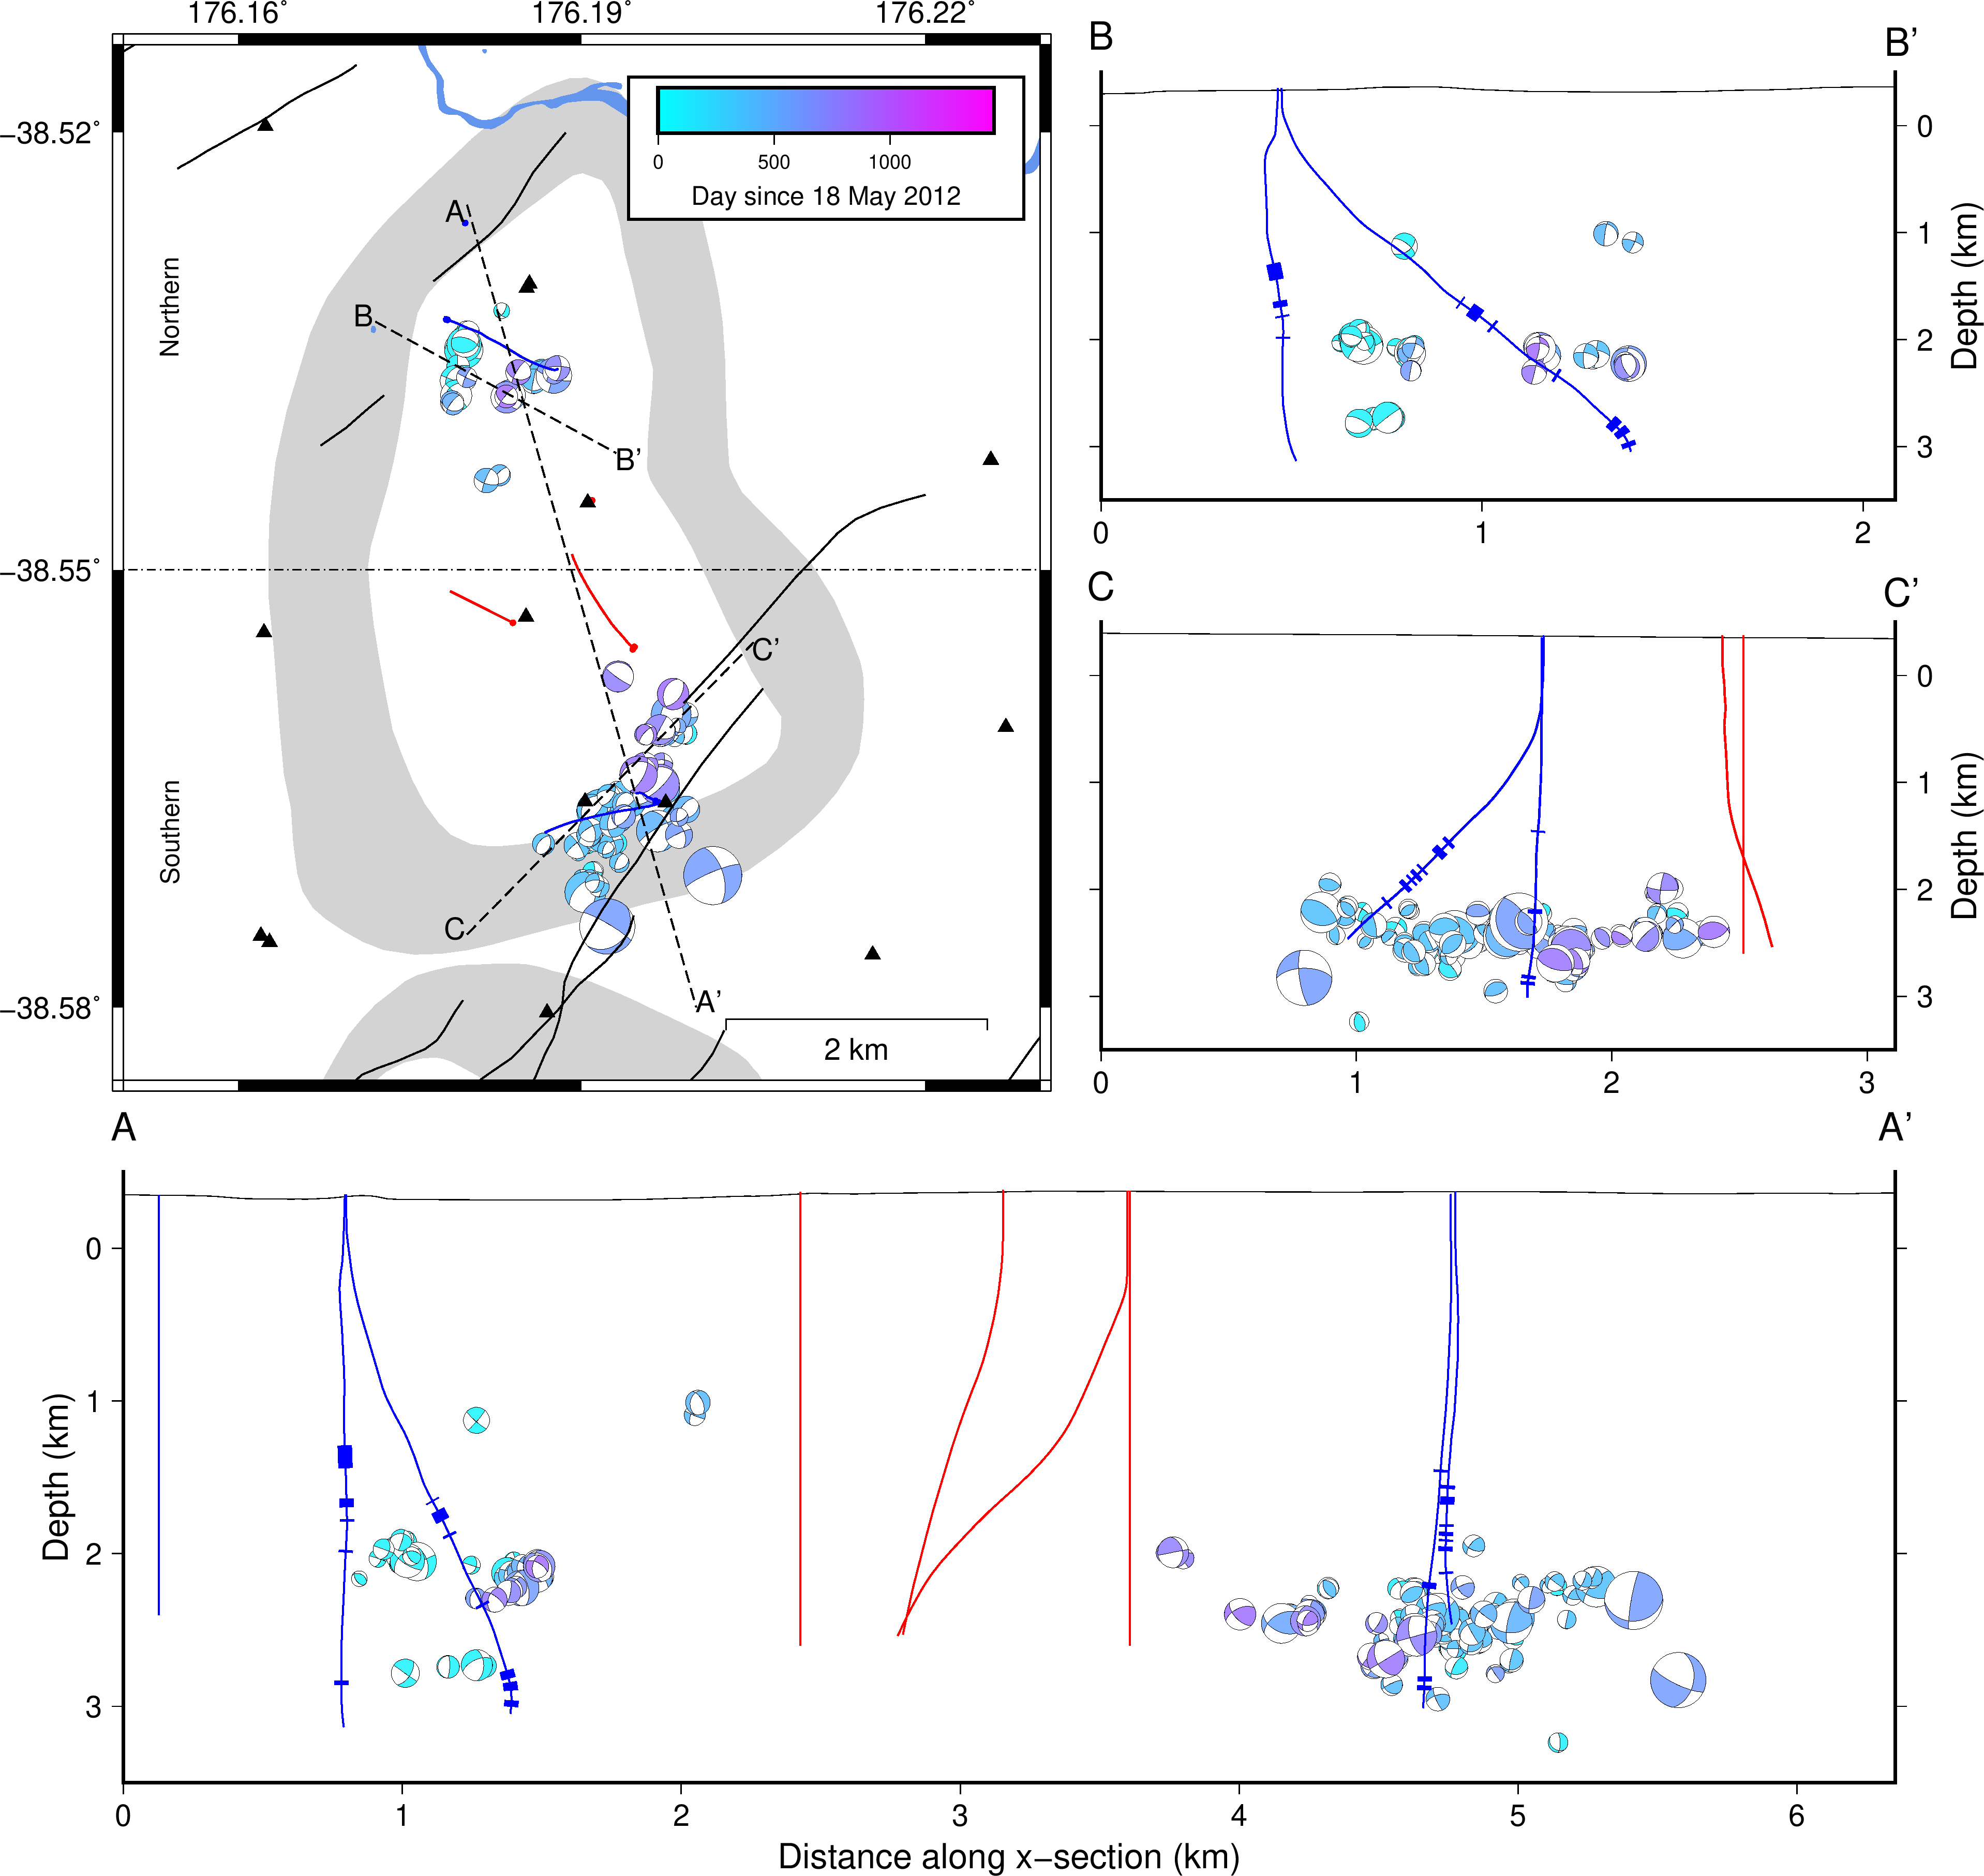
\includegraphics[width=1.00\columnwidth]{Chapter_5_FMs/figures/merc_Nga_GC_focmecs/merc_Nga_GC_focmecs_original}
\caption{{All calculated focal mechanisms for Ngatamariki from May 2012 until
November 2015. Grey polygons show the resistivity boundaries for
Ngatamariki (to the north) and Rotokawa (to the south). Black lines
indicate active faults from the GNS Active Fault Database \citep{AFDB}, red lines indicate production wells and
blue lines indicate injection wells. Focal mechanisms are colored by the
date of occurrence, with earlier events colored blue and later events
colored pink. Focal mechanisms have been reprojected in each
cross-section view to show ``back-hemisphere'' projections (i.e. the
hemisphere ``behind'' the panel). Each cross section shows only the
events within 1.5 km of the plane. Black triangles show the locations of
seismic stations.
{\label{542095}}%
}}
\end{center}
\end{figure}\selectlanguage{english}

\begin{figure}[h!]
\begin{center}
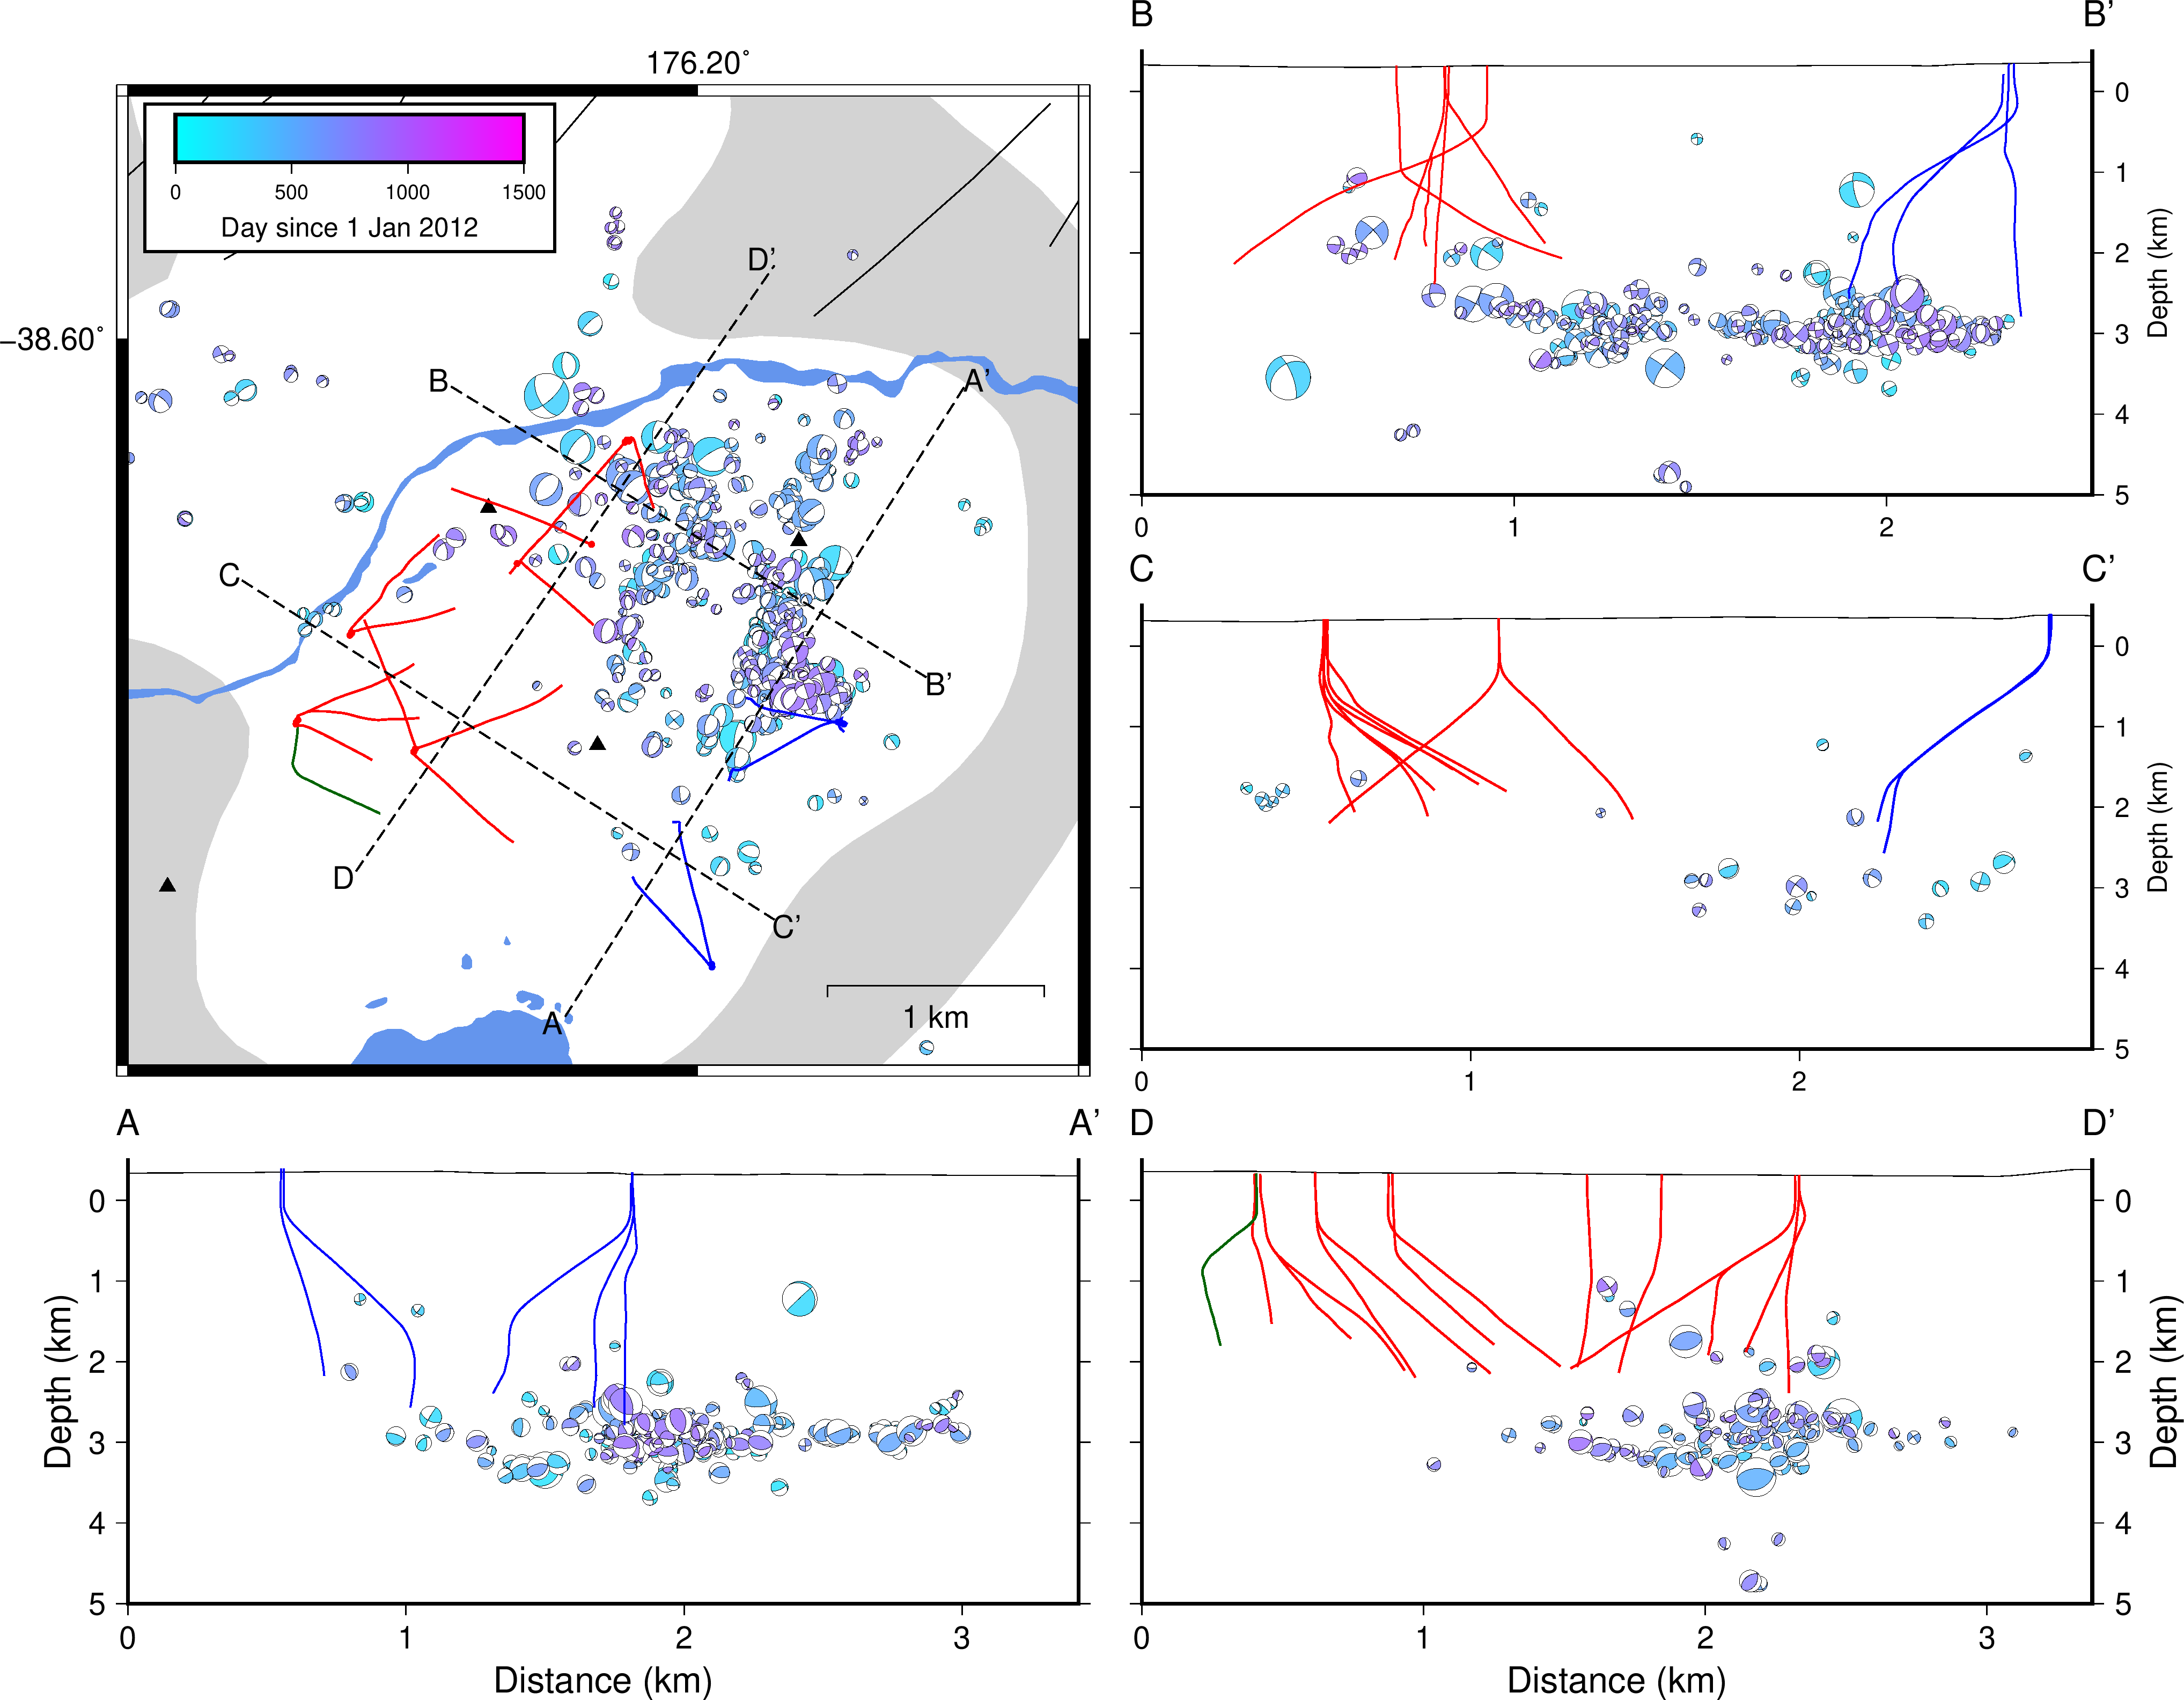
\includegraphics[width=1.00\columnwidth]{Chapter_5_FMs/figures/merc_Rot_GC_focmecs/merc_Rot_GC_focmecs_original}
\caption{{All calculated focal mechanisms for Rotokawa from May 2012 until
November 2015. The grey polygon shows the resistivity boundaries for
Rotokawa. Black lines indicate active faults from the GNS Active Fault
Database \citep{AFDB}, red lines indicate
production wells, blue lines indicate injection wells and the green line
is a reservoir monitoring well. Focal mechanisms are colored by the date
of occurrence, with earlier events colored blue and later events colored
pink. Focal mechanisms have been reprojected in each cross-section view
to show ``back-hemisphere'' projections (i.e. the hemisphere ``behind''
the panel). Each cross section shows only the events within 1.5 km of
the plane. Black triangles show the locations of seismic stations.
{\label{817909}}%
}}
\end{center}
\end{figure}

\subsection{Clustering}
\subsubsection{Correlation-based Clustering}
\subsubsection{Polarity-based Clustering}
\subsubsection{Quadtree clustering}
\subsubsection{Linearly-spaced grids}
\subsubsection{K-means Clustering}

\subsection{Stress Inversion from Focal Mechanisms}

\section{Results}
\subsection{Spatio-temporal Variations in Clusters}
\subsection{Spatio-temporal Variations in Stress}
\subsubsection{Ngatamariki: kmeans}\selectlanguage{english}

\begin{figure}[h!]
\begin{center}
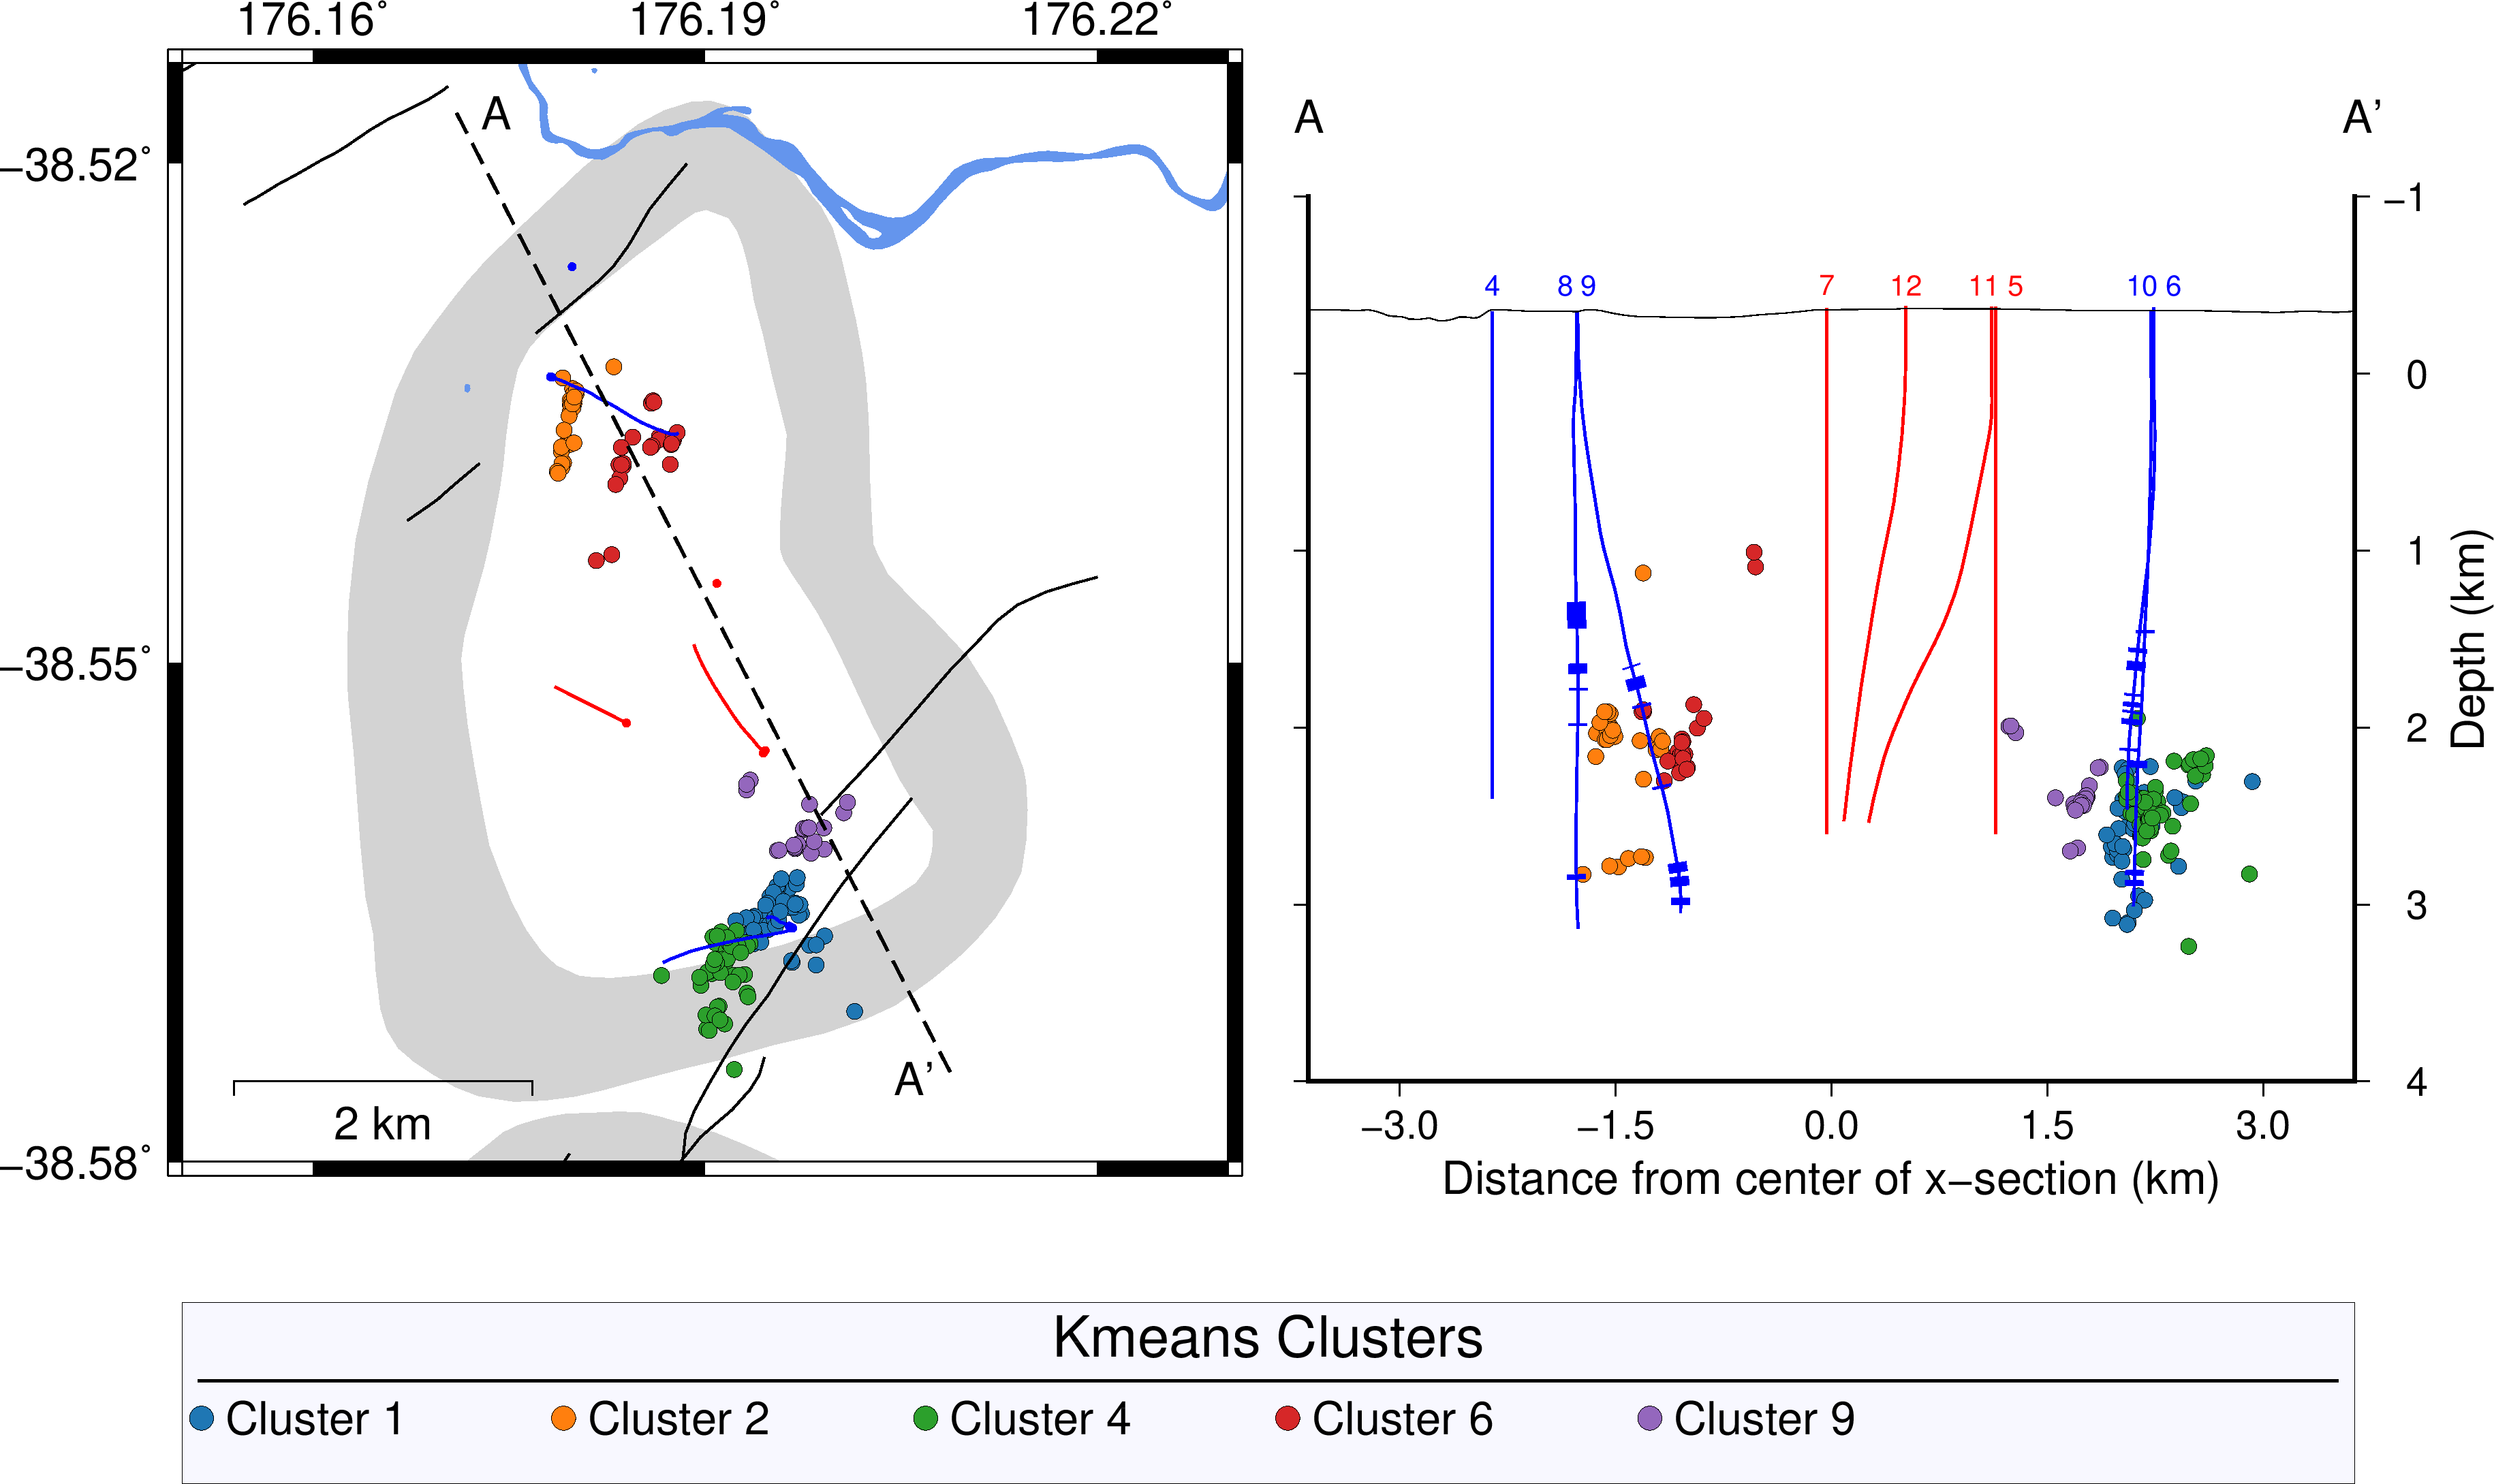
\includegraphics[width=0.98\columnwidth]{Chapter_5_FMs/figures/merc_Nga_GC_kmeans_10_GC_12-2-18/merc_Nga_kmeans_10_GC_12-2-18_original}
\caption{{Ngatamariki kmeans clusters (n=10) with greater than 20 evnets.
{\label{237918}}%
}}
\end{center}
\end{figure}\selectlanguage{english}

\begin{figure}[h!]
\begin{center}
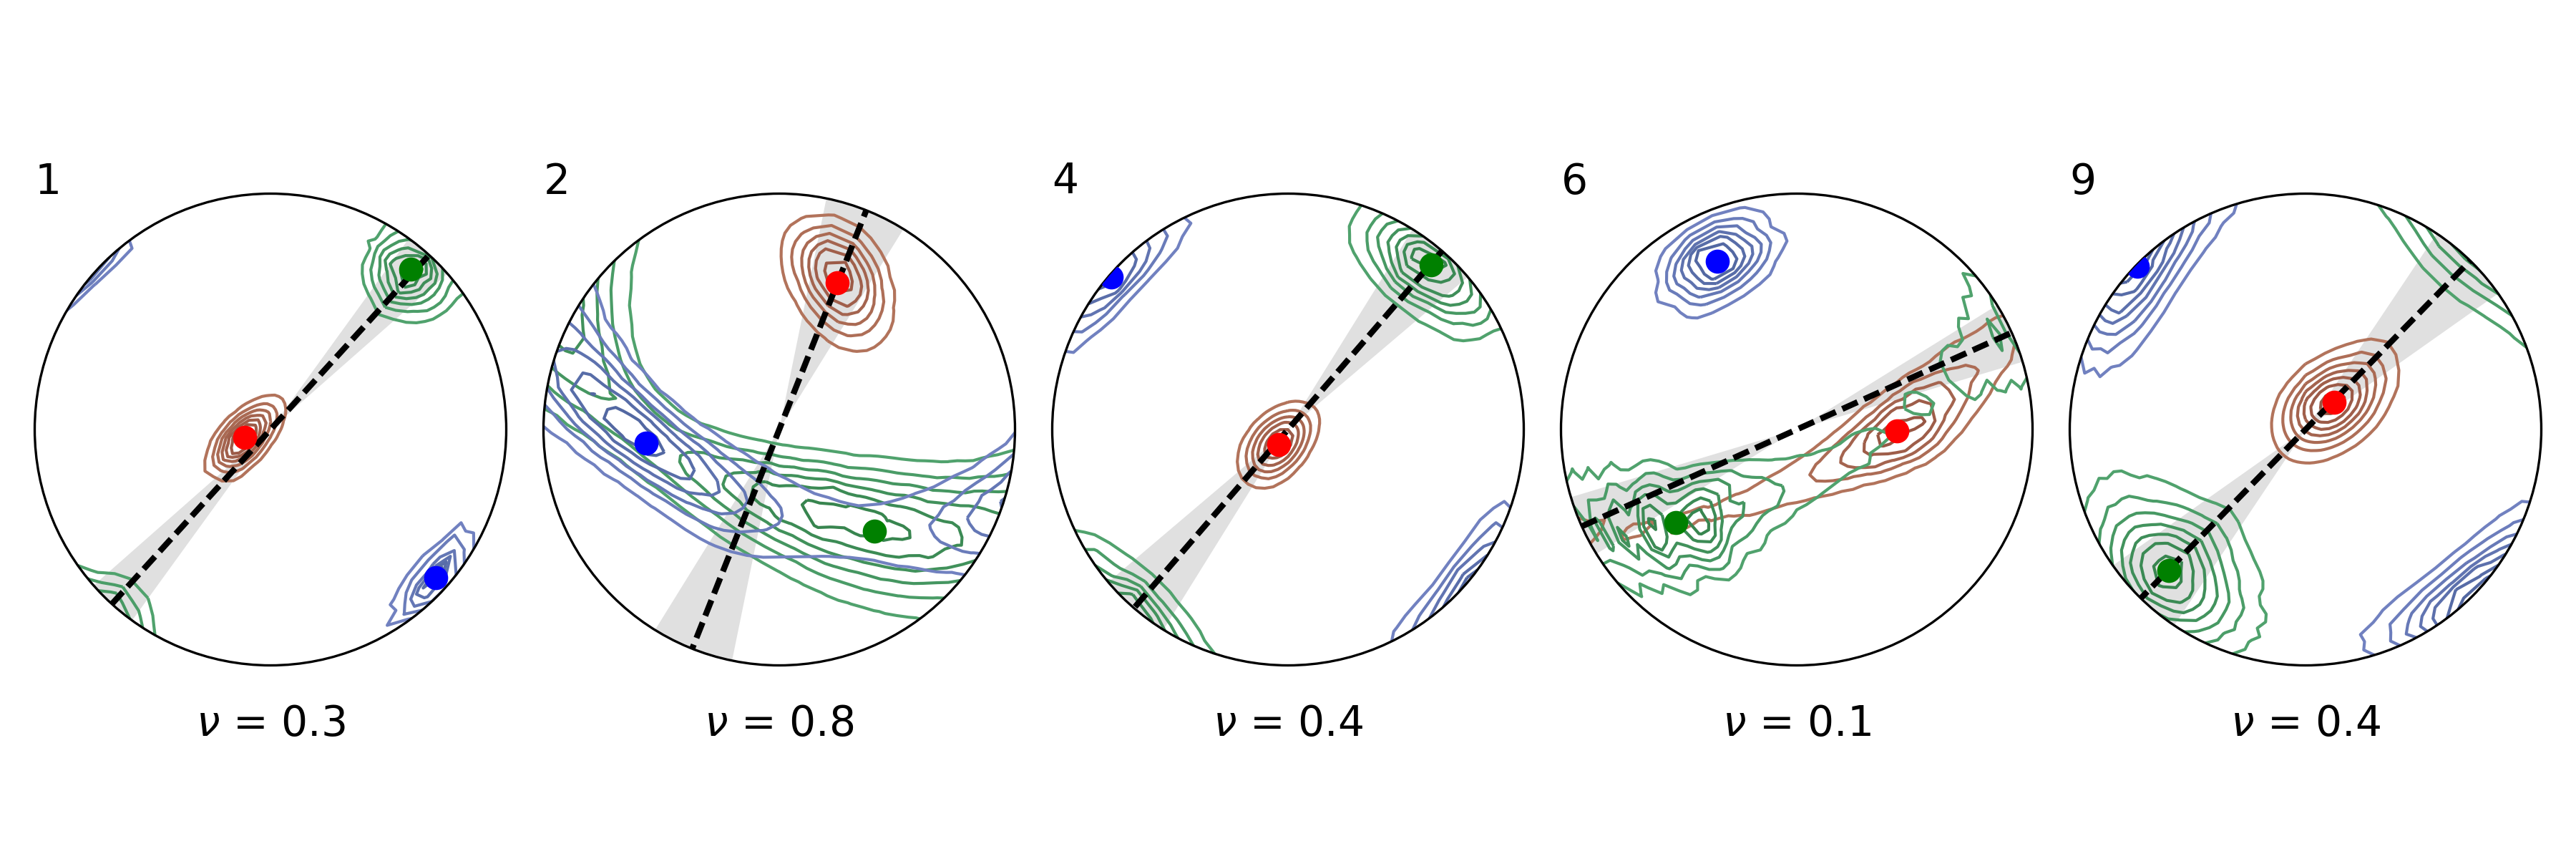
\includegraphics[width=0.98\columnwidth]{Chapter_5_FMs/figures/Nga_kmeans_inversion_10/Nga_kmeans_inversion_10_original}
\caption{{Stress inversion results for the clusters shown in
Figure~{\ref{237918}}.
{\label{838980}}%
}}
\end{center}
\end{figure}

\subsubsection{Rotokawa: kmeans}\selectlanguage{english}

\begin{figure}[h!]
\begin{center}
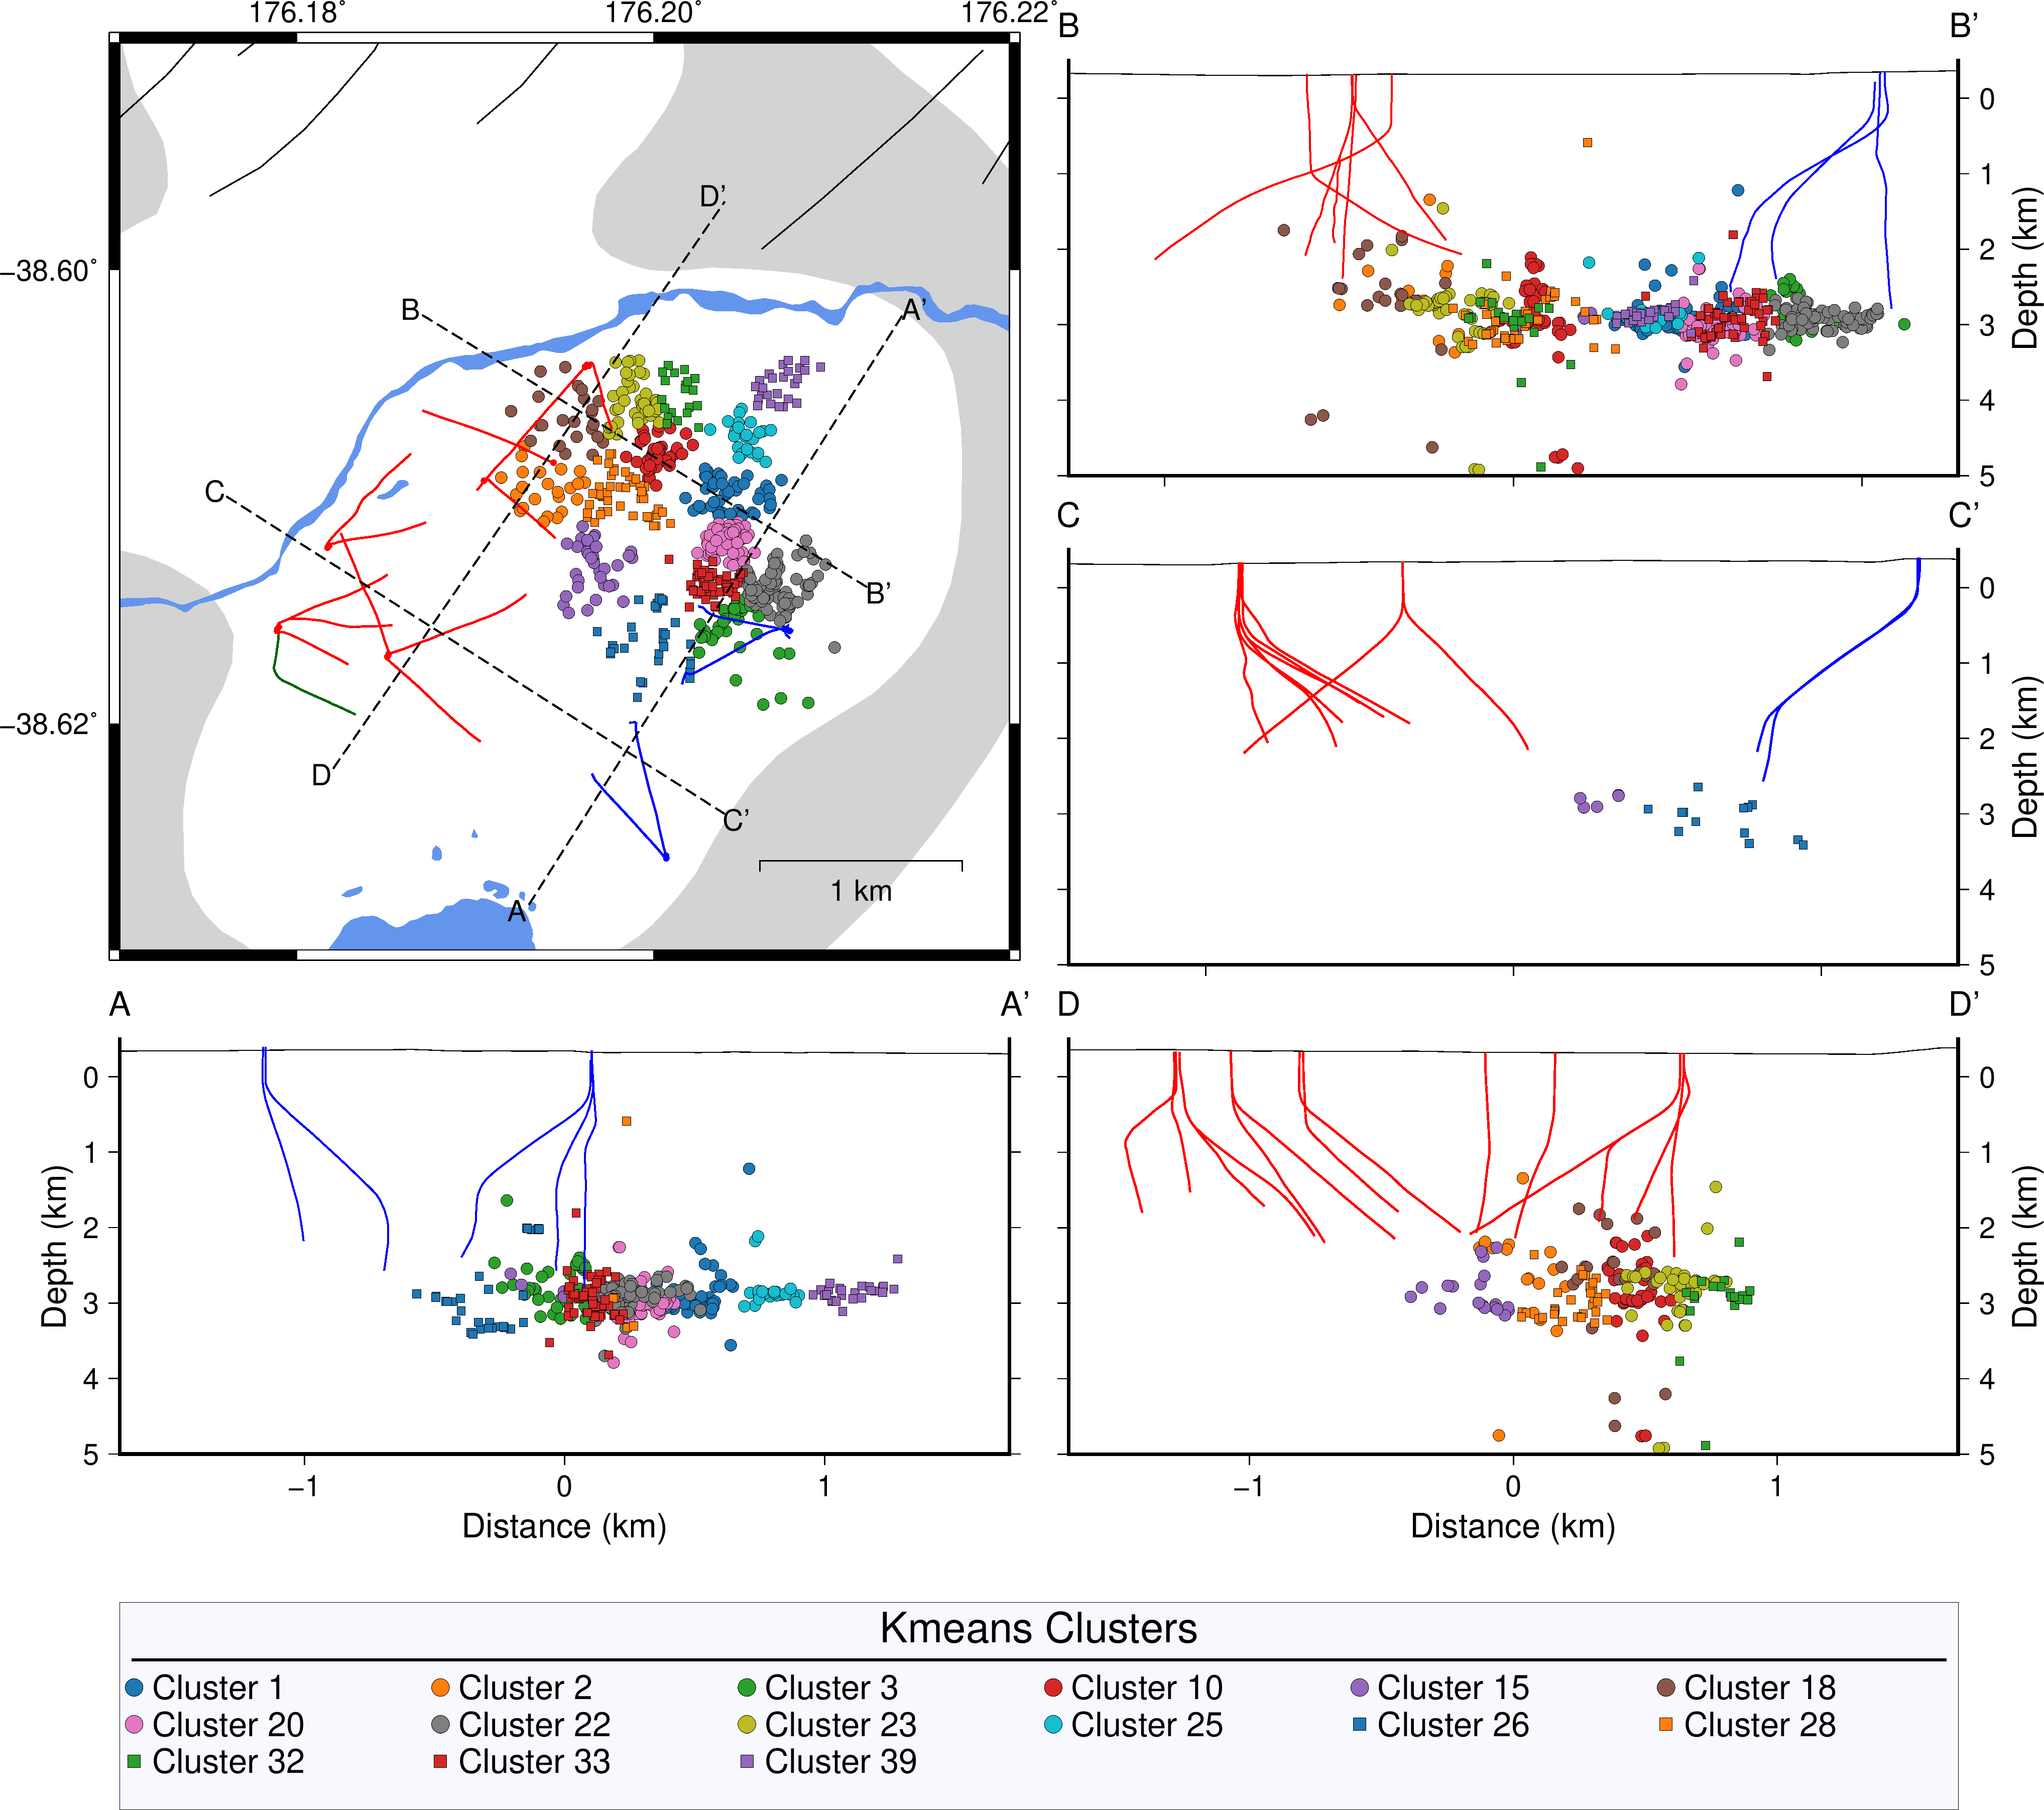
\includegraphics[width=1.00\columnwidth]{Chapter_5_FMs/figures/merc_Rot_kmeans_40/merc_Rot_kmeans_40_original}
\caption{{Rotokawa kmeans clusters (n=40) with greater than 20 events.
{\label{878143}}%
}}
\end{center}
\end{figure}\selectlanguage{english}

\begin{figure}[h!]
\begin{center}
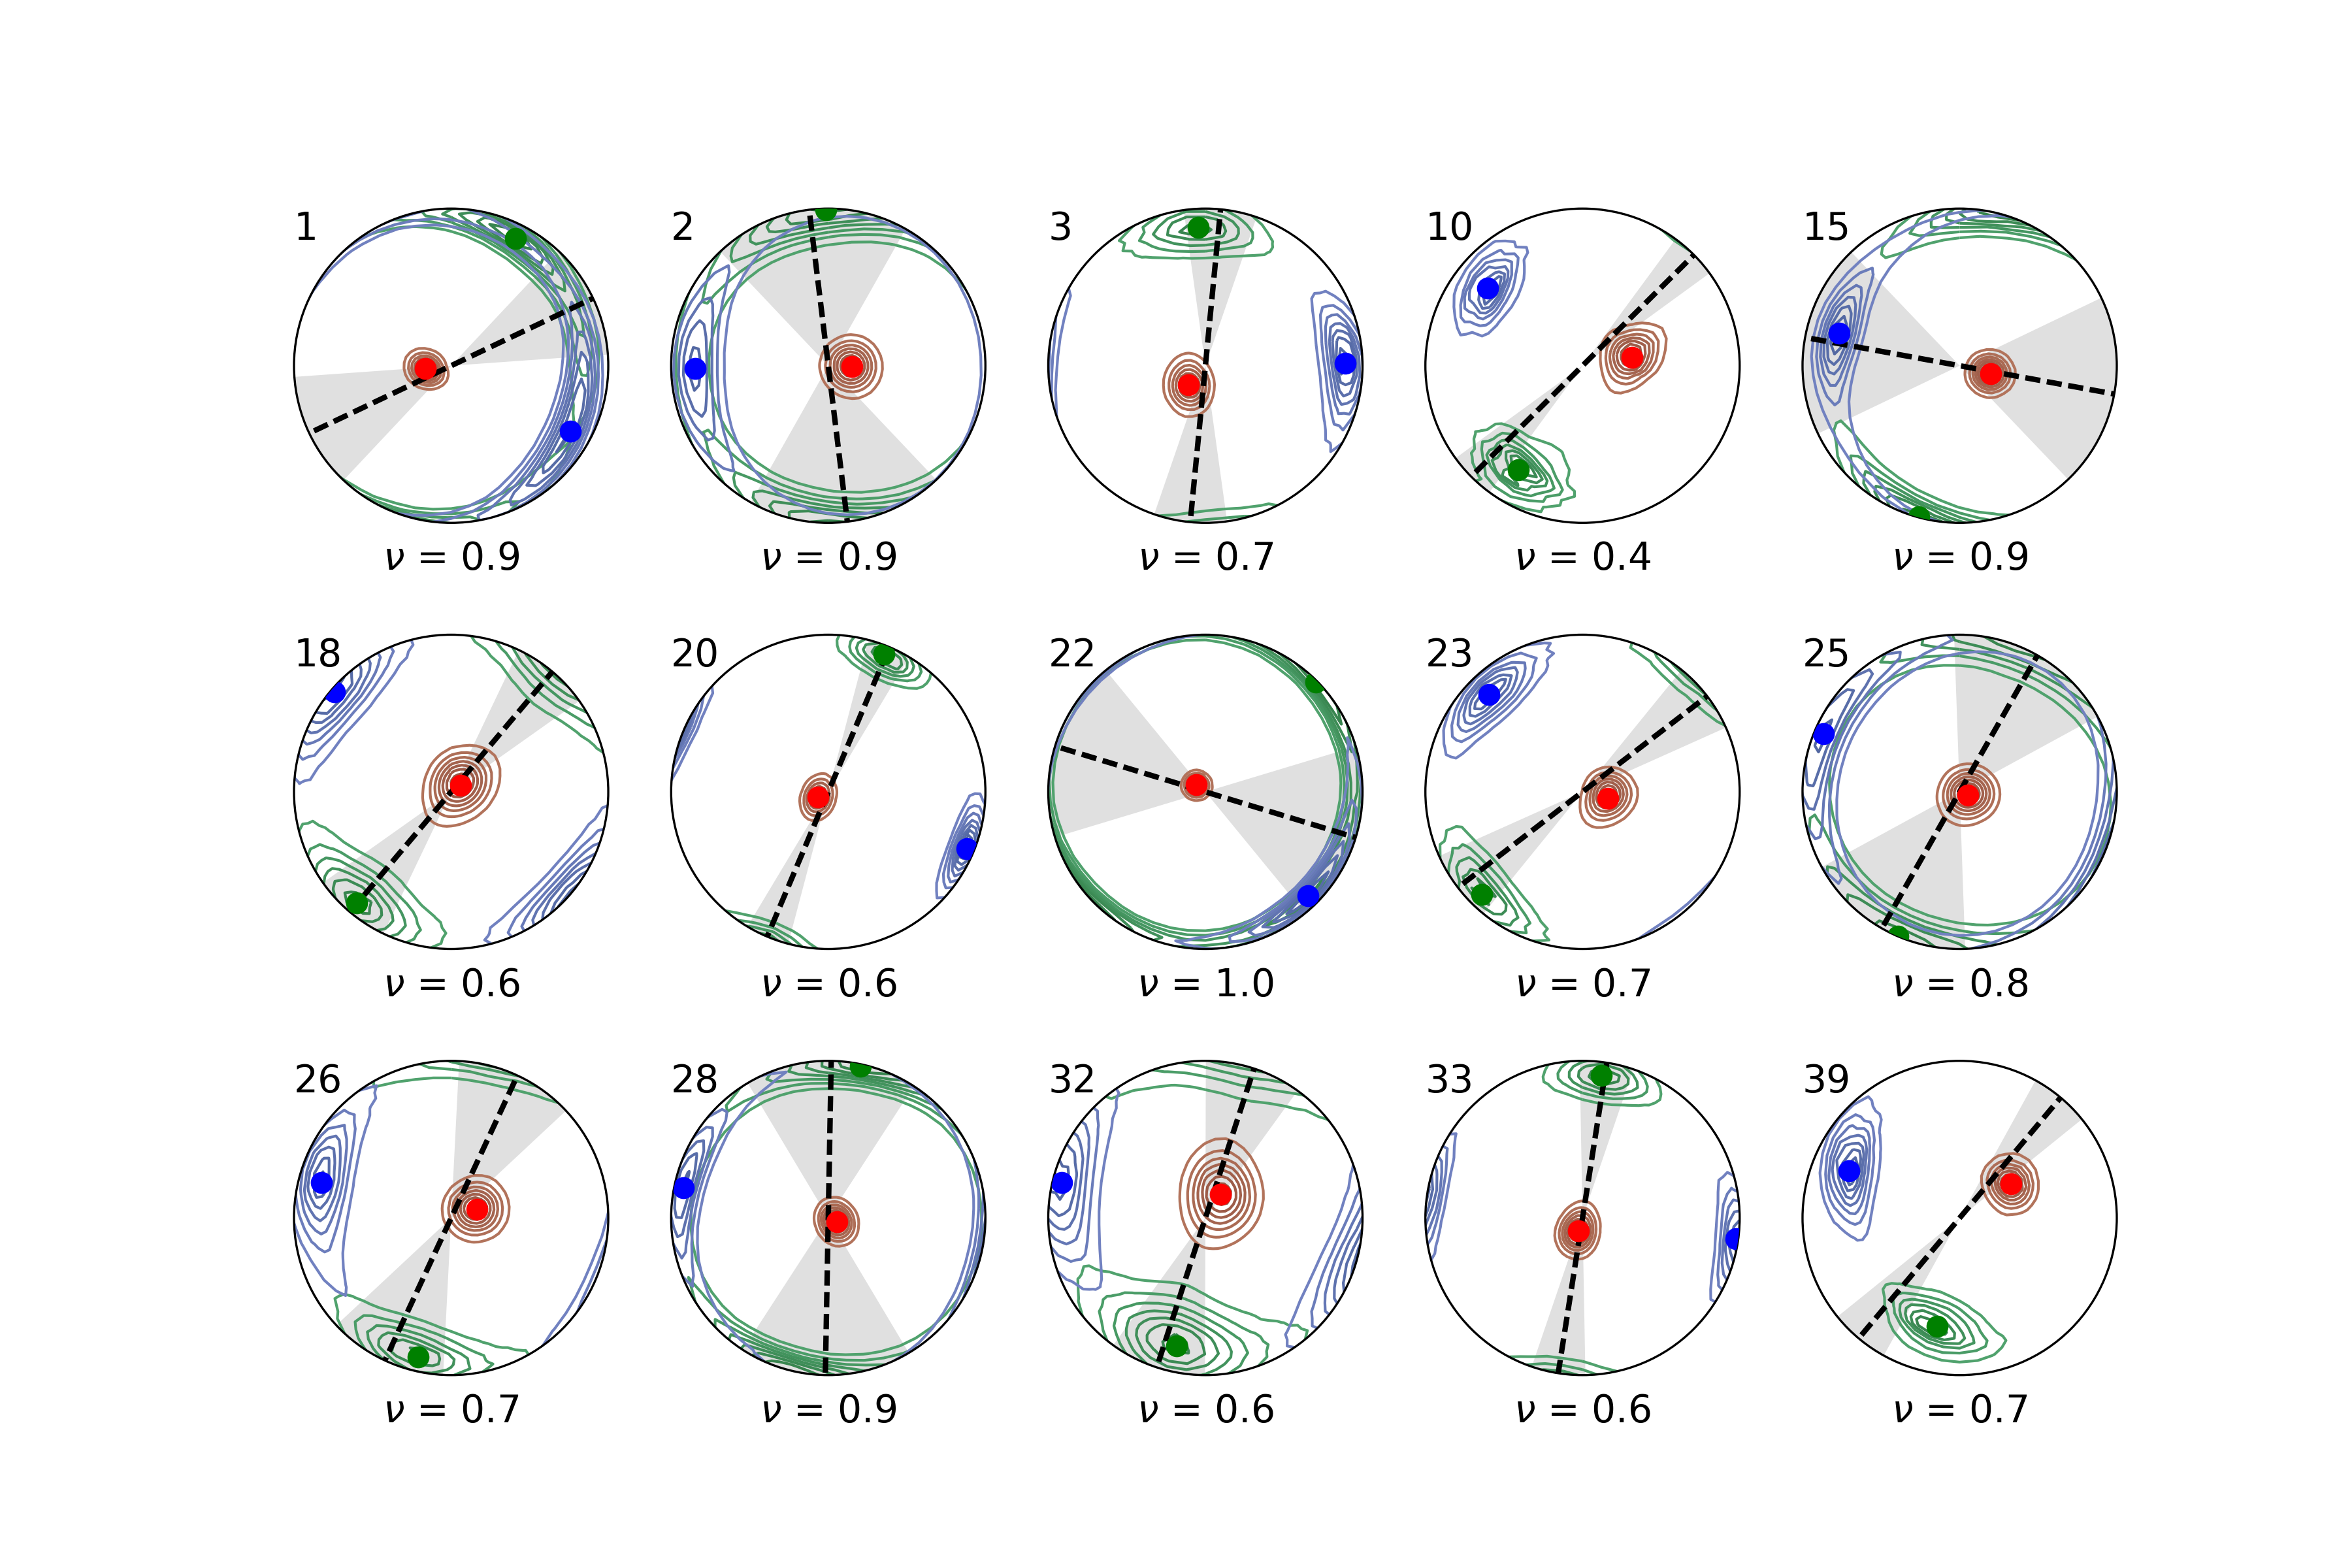
\includegraphics[width=1.00\columnwidth]{Chapter_5_FMs/figures/Rot_kmeans_inversion_40/Rot_kmeans_inversion_40_original}
\caption{{Stress inversion results corresponding to the clusters in
Figure~{\ref{878143}}.
{\label{434168}}%
}}
\end{center}
\end{figure}\selectlanguage{english}

\begin{figure}[h!]
\begin{center}
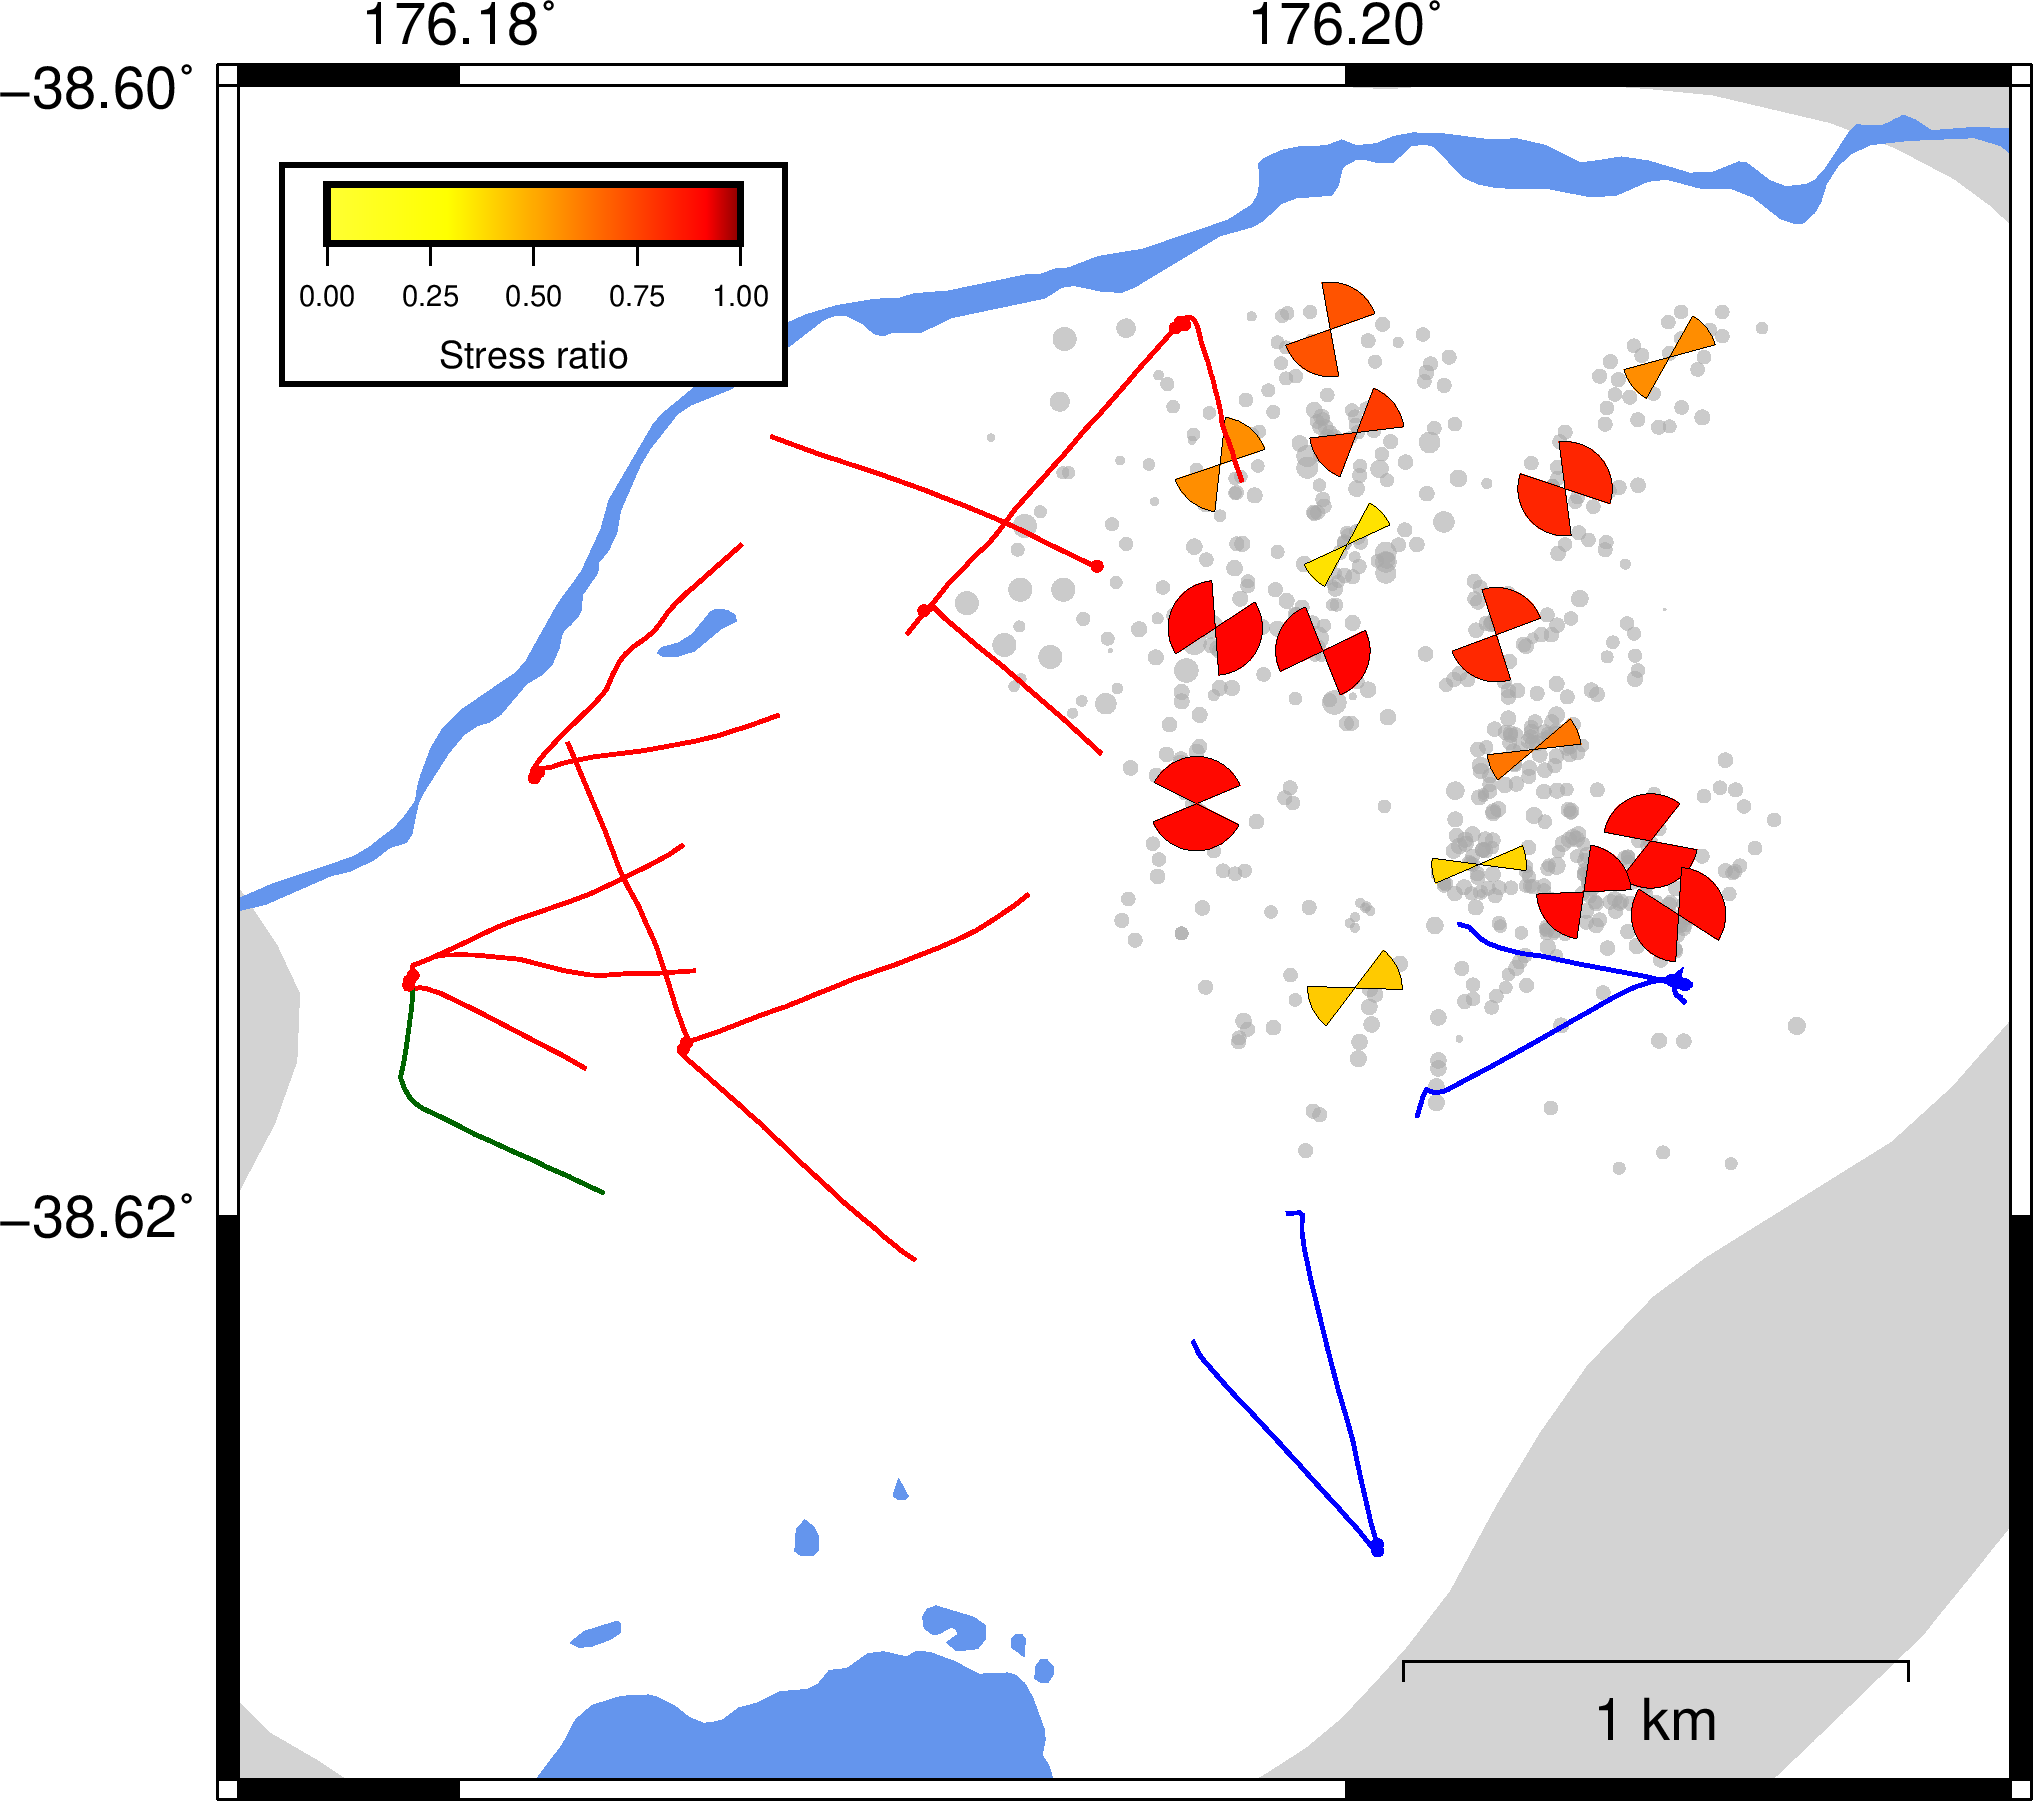
\includegraphics[width=0.84\columnwidth]{Chapter_5_FMs/figures/merc_Rot_kmeans_cents_40_sigmas_seis_nu/merc_Rot_kmeans_clust_50_cents_SHmax_nu_original}
\caption{{Principal stress directions and stress ratio for kmeans clusters (n=40)
at Rotokawa.
{\label{533041}}%
}}
\end{center}
\end{figure}

\section{Discussion and Conclusions}
\subsection{Relationship Between Clusters and Plant Operations}
\subsection{Relationship Between Stress and Injection/Production}

\section{Appendices}
\subsection{Rotokawa: Quadtree clustering}\selectlanguage{english}

\begin{figure}[h!]
\begin{center}
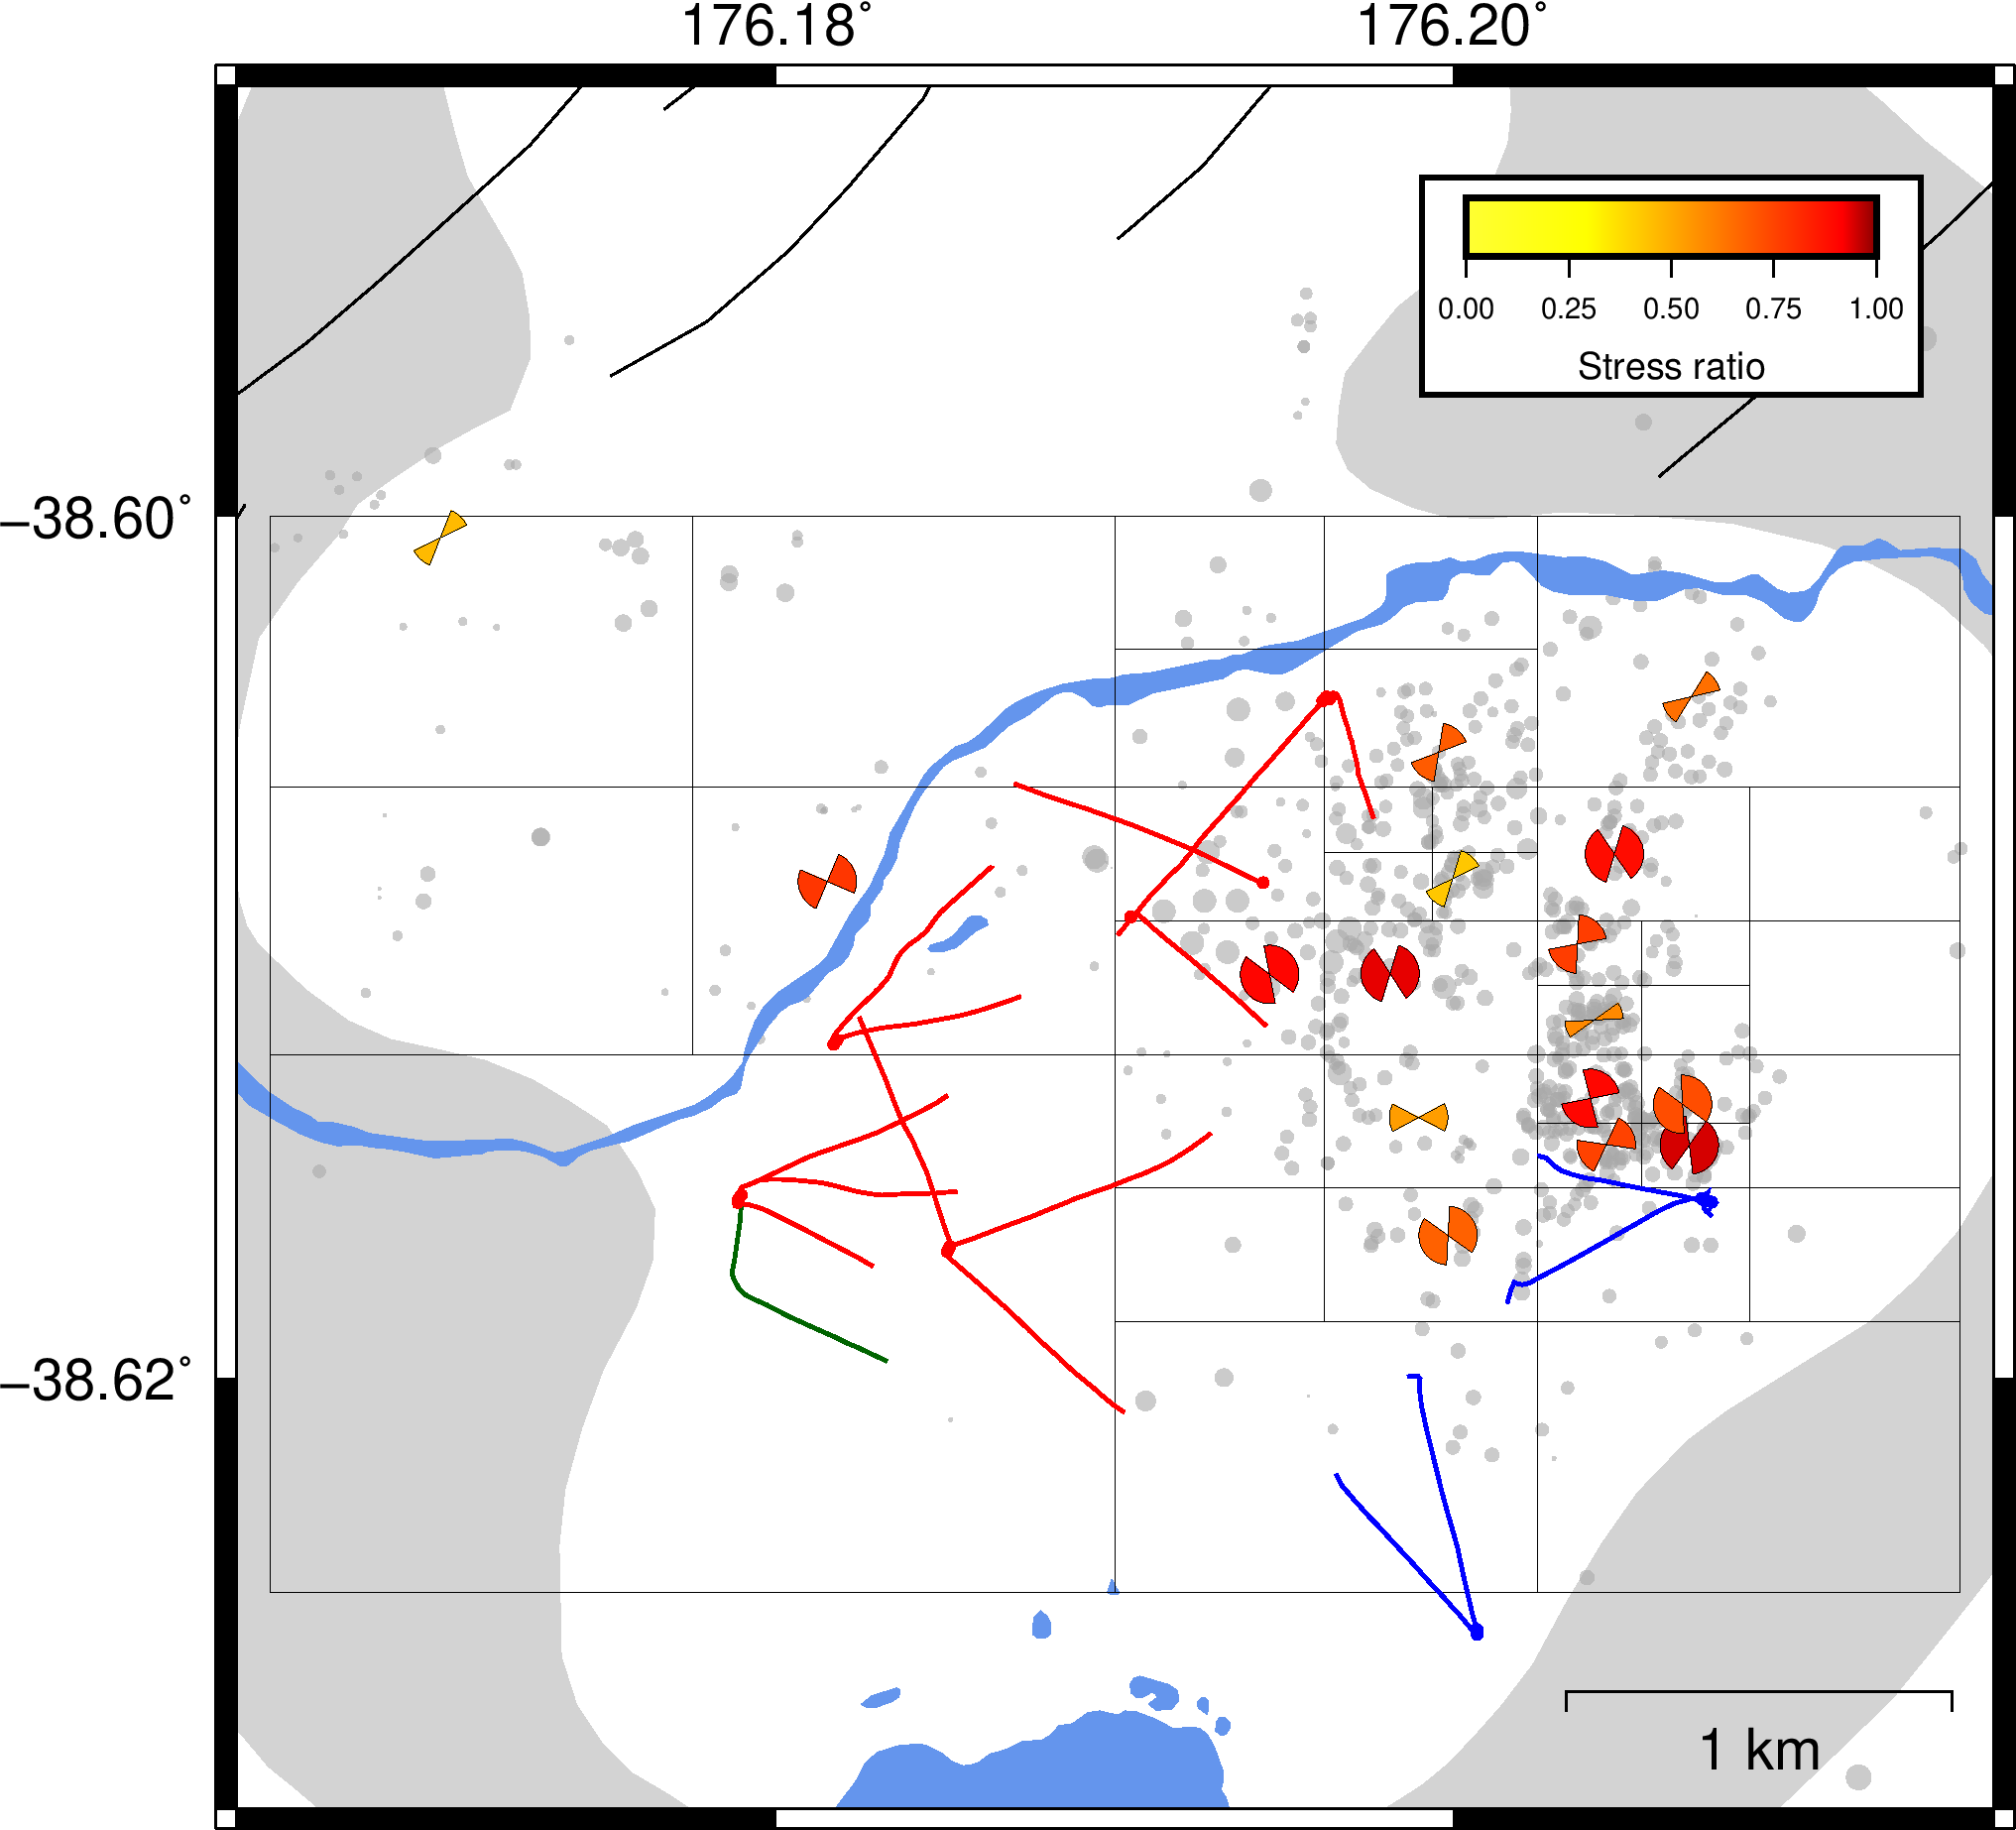
\includegraphics[width=0.84\columnwidth]{Chapter_5_FMs/figures/merc_Rot_qtree_clust_cents_sigmas/merc_Rot_qtree_clust_cents_SHmax_original}
\caption{{Principal stress directions and stress ratio for quadtree clustering
(min\_events=20, max\_events=60) of events in Rotokawa.
{\label{181502}}%
}}
\end{center}
\end{figure}

\subsection{Rotokawa: regularly-spaced grid}\selectlanguage{english}

\begin{figure}[h!]
\begin{center}
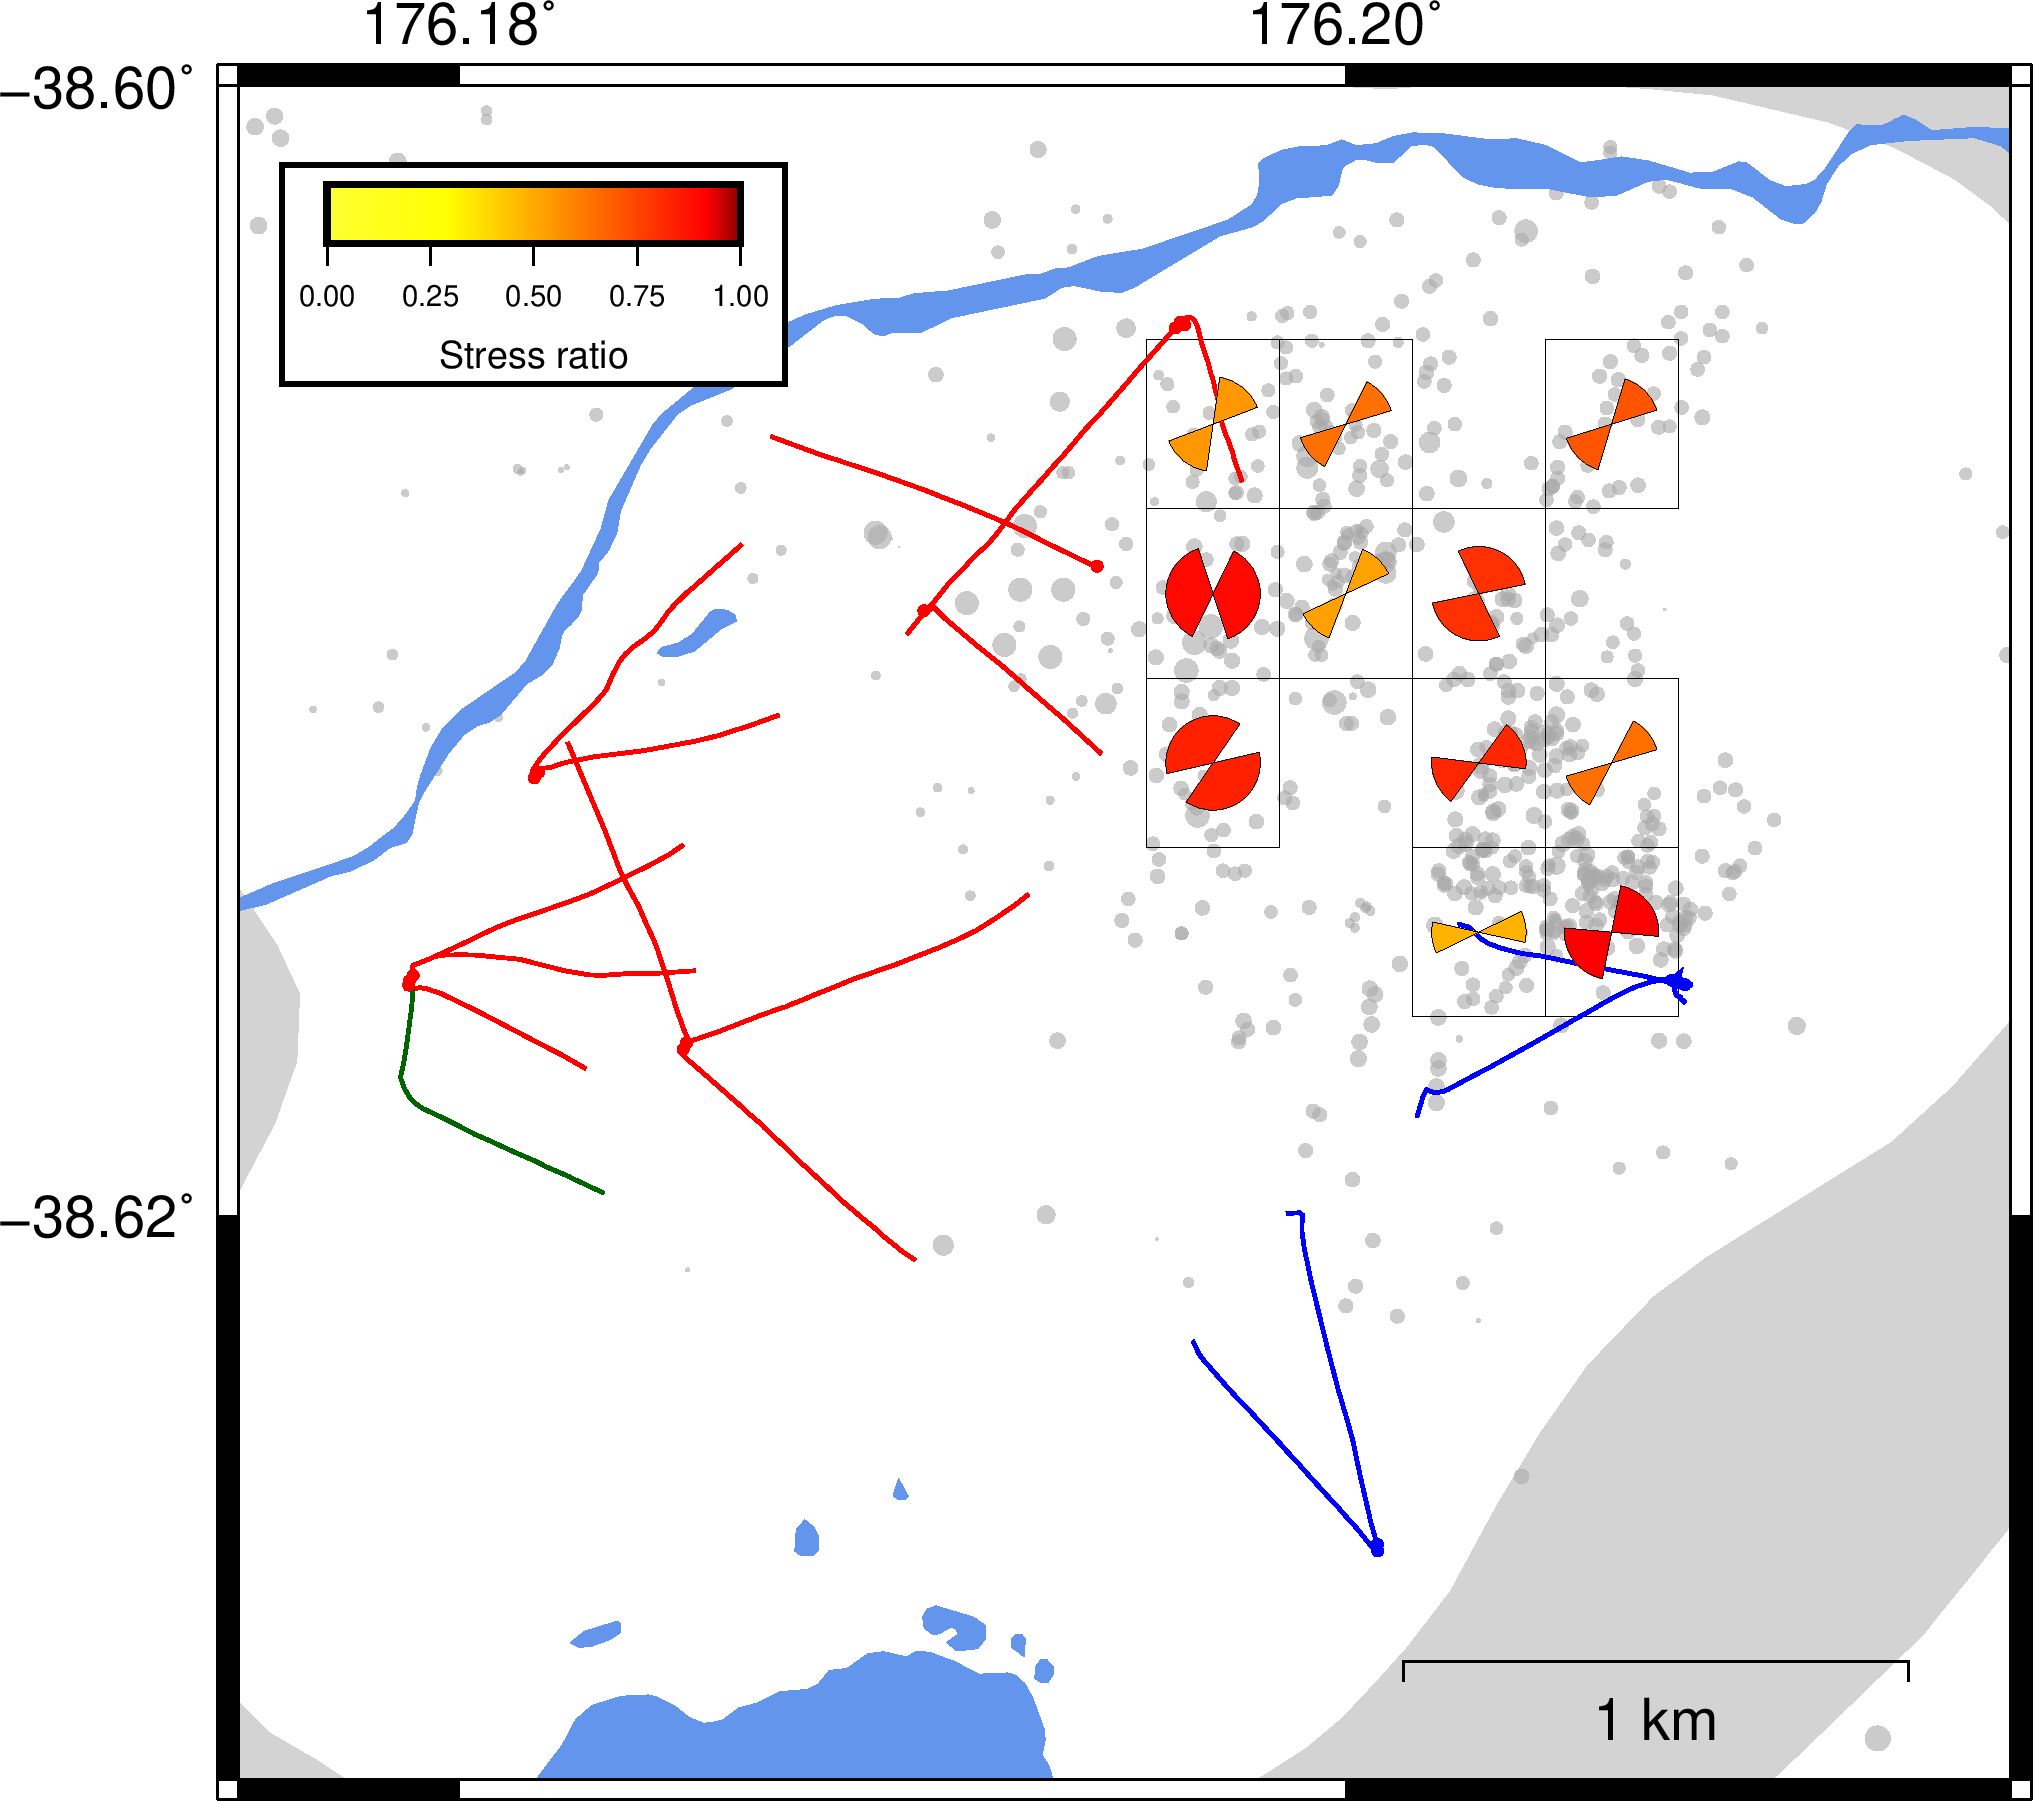
\includegraphics[width=0.84\columnwidth]{Chapter_5_FMs/figures/2D_003_sigmas/merc_Rot_2D_grid003_Arnold_clust_SHmax_nu_original}
\caption{{Stress directions and stress ratio for regularly-gridded focal
mechanisms (grid spacing=0.003 degrees), using the stress inversion
method of Arnold and Townend.~
{\label{504037}}%
}}
\end{center}
\end{figure}\selectlanguage{english}

\begin{figure}[h!]
\begin{center}
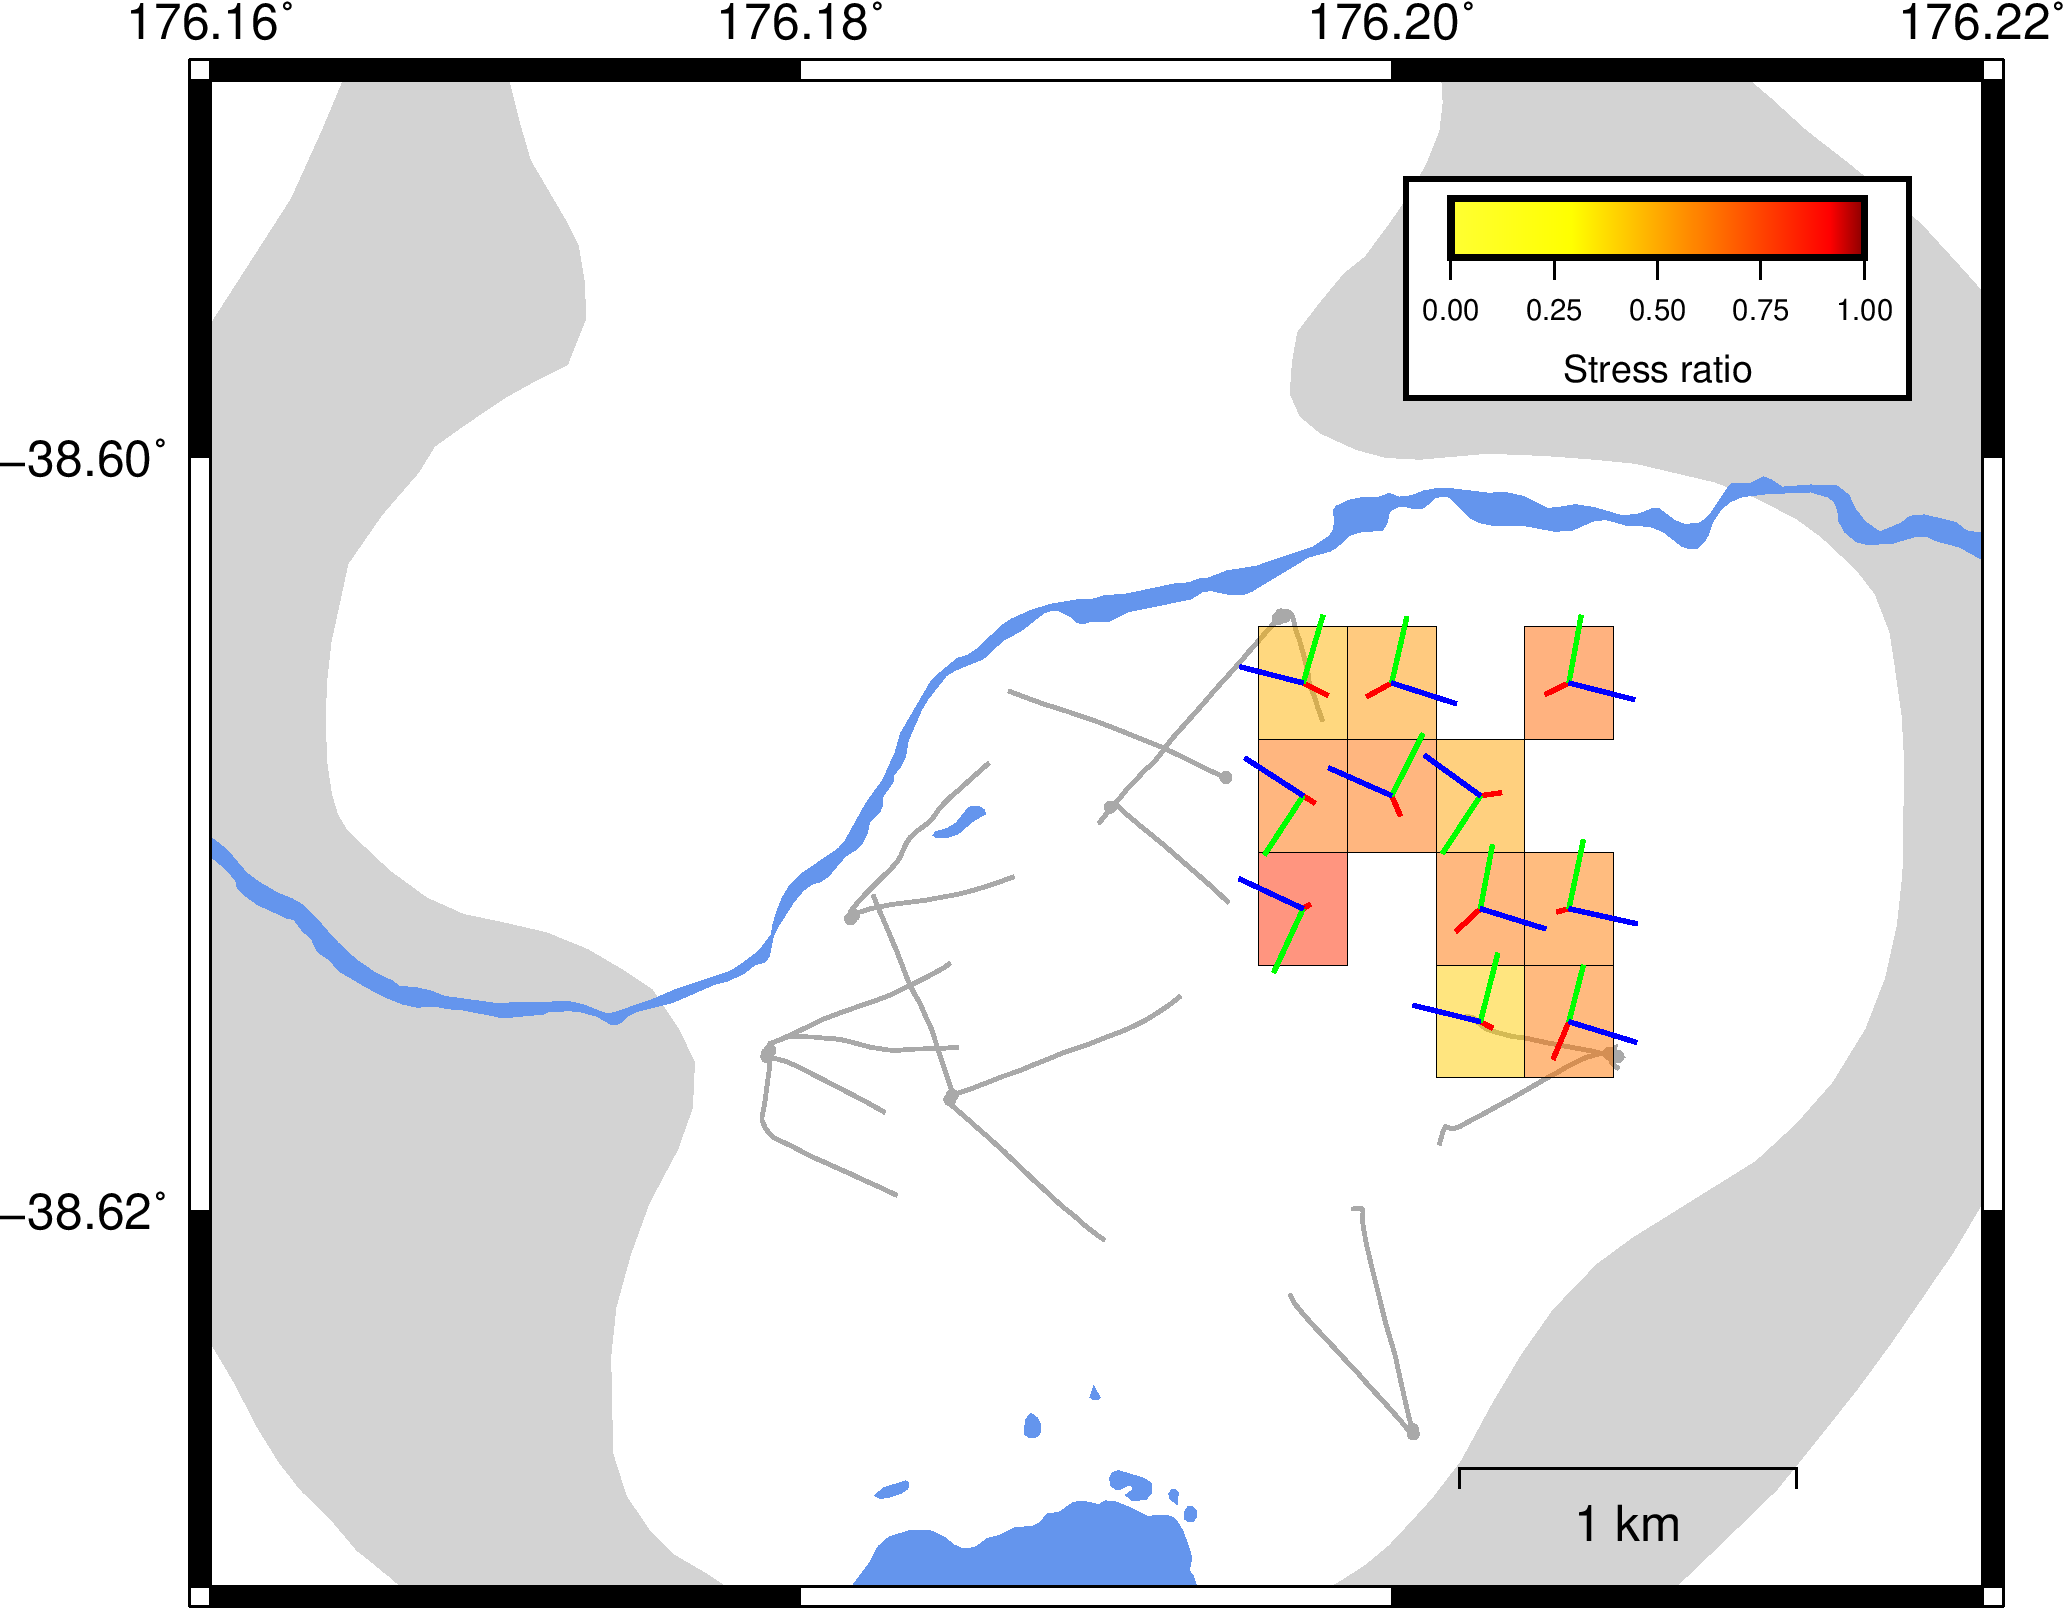
\includegraphics[width=0.84\columnwidth]{Chapter_5_FMs/figures/merc_Rot_msatsi_003_2D/merc_Rot_msatsi_003_2D_original}
\caption{{Directions of the three principle stresses (\(\sigma_1\)
=red,~\(\sigma_2\) =green,~\(\sigma_3\) =red) for the same
gridded clusters as Figure~{\ref{504037}} above using
the MSATSI inversion program of Martinez-Garzon and Hardebeck.
{\label{317691}}%
}}
\end{center}
\end{figure}